\immediate\write18{makeindex \jobname.nlo -s nomencl.ist -o \jobname.nls}
%%%%%%%%%%%%%%%%%%%%%%%%%%%%%%%%%%%%%%%%%%%%%%%%%%%%%%%%%%%%%%%
%% OXFORD THESIS TEMPLATE

%%%%%%%%
%pdflatex --shell-escape thesis
%biber
%pdflatex --shell-escape thesis
%pdflatex --shell-escape thesis

%%%%%%%


% Use this template to produce a standard thesis that meets the Oxford University requirements for Dcsubmission
%
% Originally by Keith A. Gillow (gillow@maths.ox.ac.uk), 1997
% Modified by Sam Evans (sam@samuelevansresearch.org), 2007
% Modified by John McManigle (mcmanigle@gmail.com), 2015
% Modified by Martin Peeks (martinp23@gmail.com), 2017

% I've (John) tried to comment this file extensively, so read through it to see how to use the various options.  Remember
% that in LaTeX, any line starting with a % is NOT executed.  Several places below, you have a choice of which line to use
% out of multiple options (eg draft vs final, for PDF vs for binding, etc.)  When you pick one, add a % to the beginning of
% the lines you don't want.

% I (Martin) have perhaps been less good at commenting, so apologies.
% I have added to biber.conf lots of find/replace statements to change journal names into journal abbreviations. You might need to add more patterns there if you add other journals to your bibliography.
% Because I removed several chapters from this version for upload to github, some cross-references are broken.

%%%%% CHOOSE PAGE LAYOUT
% The most common choices should be below.  You can also do other things, like replacing "a4paper" with "letterpaper", etc.

% This one will format for two-sided binding (ie left and right pages have mirror margins; blank pages inserted where needed):
%\RequirePackage{snapshot}
\documentclass[a4paper,twoside]{ociamthesis}
\usepackage[export]{adjustbox}



\usepackage[T1]{fontenc}
\usepackage{textgreek}
% This one will format for one-sided binding (ie left margin > right margin; no extra blank pages):
%\documentclass[a4paper]{ociamthesis}
% This one will format for PDF output (ie equal margins, no extra blank pages):
%\documentclass[a4paper,nobind]{ociamthesis}


%%%%% SELECT YOUR DRAFT OPTIONS
% Three options going on here; use in any combination.  But remember to turn the first two off before
% generating a PDF to send to the printer!

% This adds a "DRAFT" footer to every normal page.  (The first page of each chapter is not a "normal" page.)
%\fancyfoot[C]{\emph{DRAFT Printed on \today}}



% This highlights (in blue) corrections marked with (for words) \mccorrect{blah} or (for whole
% paragraphs) \begin{mccorrection} . . . \end{mccorrection}.  This can be useful for sending a PDF of
% your corrected thesis to your examiners for review.  Turn it off, and the blue disappears.
%%\correctionstrue


%%%%% BIBLIOGRAPHY SETUP
% Note that your bibliography will require some tweaking depending on your department, preferred format, etc.
% The options included below are just very basic "sciencey" and "humanitiesey" options to get started.
% If you've not used LaTeX before, I recommend reading a little about biblatex/biber and getting started with it.
% If you're already a LaTeX pro and are used to natbib or something, modify as necessary.
% Either way, you'll have to choose and configure an appropriate bibliography format...

% The science-type option: numerical in-text citation with references in order of appearance.
\usepackage[style=chem-rsc,articletitle=true,language=british,backend=biber]{biblatex}
\newcommand*{\bibtitle}{References}

% show title for a thesis
\DeclareBibliographyDriver{thesis}{%
  \usebibmacro{bibindex}%
  \usebibmacro{begentry}%
  \usebibmacro{author}%
  \setunit{\labelnamepunct}%\newblock
  %\printlist{language}%
  \newunit\newblock
  \usebibmacro{byauthor}%
  \newunit\newblock%Added by Marco
  \usebibmacro{title}%Added by Marco
  \newunit\newblock
  \printfield{note}%
  \newunit\newblock
  \printfield{type}%
  \newunit
  \usebibmacro{institution+location+date}%
  \newunit\newblock
  \usebibmacro{chapter+pages}%
  \newunit
  \printfield{pagetotal}%
  \newunit\newblock
  \iftoggle{bbx:isbn}
    {\printfield{isbn}}
    {}%
  \newunit\newblock
  \usebibmacro{doi+eprint+url}%
  \newunit\newblock
  \usebibmacro{addendum+pubstate}%
  \setunit{\bibpagerefpunct}\newblock
  \usebibmacro{pageref}%
  \usebibmacro{finentry}%
}


% correctly format an online reference
\DeclareBibliographyDriver{online}{%
  \usebibmacro{bibindex}%
  \usebibmacro{begentry}%
  \iflistundef{author}
    {\iflistundef{organization}
      {\BibliographyWarning{No author nor organisation on Online entry}}
      {\printlist{organization}}}
    {\usebibmacro{author}}
  \setunit{\labelnamepunct}\newblock
  \usebibmacro{title}%
  \newunit
  \printlist{language}%
  \newunit\newblock
  \usebibmacro{byauthor}%
  \newunit\newblock
  \usebibmacro{byeditor+others}%
  \newunit\newblock
  \printfield{version}%
  \newunit
  \printfield{note}%
  \newunit\newblock
  \iflistundef{author}
    {}
    {\printlist{organization}}
  \newunit\newblock
  \usebibmacro{date}%
  \newunit\newblock
  \iftoggle{bbx:eprint}
    {\usebibmacro{eprint}}
    {}%
  \newunit\newblock
  \usebibmacro{url+urldate}%
  \newunit\newblock
  \usebibmacro{addendum+pubstate}%
  \setunit{\bibpagerefpunct}\newblock
  \usebibmacro{pageref}%
  \usebibmacro{finentry}}



% if showing a full citation in line, display it correctly
\preto\fullcite{\AtNextCite{\defcounter{maxnames}{99}}}


% remove brackets around the number of each bibliography entry
\DeclareFieldFormat{labelnumberwidth}{#1\addperiod}


% \renewbibmacro*{title}{
%   \ifentrytype{article}% Delimit article and journal titles with a period
%     {\adddot}
%     {}}
\usepackage{graphicx} % so we can put pdf figures in
\usepackage[runs=1]{auto-pst-pdf} % necessary for chemnum. Formally, runs=2 should be used. I had more success running pdflatex twice.
%\usepackage{chemstyle}
\usepackage{xspace}
\usepackage{imakeidx}
% The humanities-type option: author-year in-text citation with an alphabetical works cited.
%\usepackage[style=authoryear, sorting=nyt, backend=biber, maxcitenames=2, useprefix, doi=false, isbn=false]{biblatex}
%\newcommand*{\bibtitle}{Works Cited}\cmd{}
\usepackage{multirow}
\usepackage{array}
\usepackage{arydshln}
\usepackage{chemnum}
\usepackage{siunitx}
\usepackage{subfig}
\usepackage{pdflscape}
\usepackage{rotating}
\usepackage[intoc]{nomencl}
\usepackage{multicol}
\renewcommand{\nomname}{List of Abbreviations}
\usepackage{placeins}
\usepackage{longtable}
\raggedbottom

% chemnum config
\setchemnum{replace-style={\scriptsize}}
\setchemnum{log=true}
% this makes compound labels all red, useful for checking
%\setchemnum{replace-style={\scriptsize\color{red}},format={\color{red}\bfseries}}

%\usepackage{setspace}
%\doublespacing

% set my preferred footnote symbol
\renewcommand{\thefootnote}{\fnsymbol{footnote}}

% This makes the bibliography left-aligned (not 'justified') and slightly smaller font.
\renewcommand*{\bibfont}{\raggedright\small}
%\renewcommand{\cite}{\autocite}

%\appto{\bibsetup}{\sloppy}
% Change this to the name of your .bib file (usually exported from a citation manager like Zotero or EndNote).
\addbibresource{thesis.bib}


% Uncomment this if you want equation numbers per section (2.3.12), instead of per chapter (2.18):
%\numberwithin{equation}{subsection}



%%%%% THESIS / TITLE PAGE INFORMATION
% Everybody needs to complete the following:
\title{Electronic delocalisation in linear and cyclic porphyrin oligomers}
\author{Martin D. Peeks}
\college{Exeter College}

% Master's candidates who require the alternate title page (with candidate number and word count)
% must also un-comment and complete the following three lines:
%\masterssubmissiontrue
%\candidateno{933516}
%\wordcount{28,815}

% Uncomment the following line if your degree also includes exams (eg most masters):
%\renewcommand{\submittedtext}{Submitted in partial completion of the}
% Your full degree name.  (But remember that DPhils aren't "in" anything.  They're just DPhils.)
\degreename{Doctor of Philosophy}
% Term and year of submission, or date if your board requires (eg most masters)
\degreedate{Michaelmas 2016}


%%%%% YOUR OWN PERSONAL MACROS
% This is a good place to dump your own LaTeX macros as they come up.

% To make text superscripts shortcuts
%%	\renewcommand{\th}{\textsuperscript{th}} % ex: I won 4\th place
%%	\newcommand{\nd}{\textsuperscript{nd}}
%%	\renewcommand{\st}{\textsuperscript{st}}
%%	\newcommand{\rd}{\textsuperscript{rd}}

% I am leaving this dump of thesis-specific macros here. Delete them if you don't need them.

\DeclareSIUnit\molar{\mole\per\cubic\deci\metre}
\DeclareSIUnit\Molar{M}
\DeclareSIUnit\ppm{ppm}
\DeclareSIUnit\wn{\per\centi\metre}
\DeclareSIUnit\bohr{bohr}
\DeclareSIUnit\litre{L}
\DeclareSIUnit\mm{\milli\metre}
\DeclareSIUnit\mL{\milli\litre}
\DeclareSIUnit\ml{\milli\litre}
\DeclareSIUnit\mmol{\milli\mole}
\DeclareSIUnit\mM{\milli\Molar}
\DeclareSIUnit\umol{\micro\mole}
\DeclareSIUnit\ul{\micro\litre}
\DeclareSIUnit\uL{\micro\litre}
\DeclareSIUnit\kjmol{\kilo\joule\per\mole}
\DeclareSIUnit\jkmol{\joule\per\kelvin\per\mole}


\setlength{\headheight}{27.185pt}

\newcommand{\textcal}[1]{{\fontfamily{pzc}\selectfont#1}}
\newcommand{\pol}[1]{{P}\tsub{#1}}
\newcommand{\lp}[1]{\mbox{\textbf{\textit{l}-P{#1}}}}
\newcommand{\cp}[1]{\mbox{\textbf{\textit{c}-P{#1}}}}
\newcommand{\tp}[1]{\mbox{\textbf{\textit{t}-P{#1}}}}
\newcommand{\tubewt}{\mbox{\textbf{\textit{t}-P12{$\bullet{}$T6\textsubscript{2}}}}}
\newcommand{\p}[1]{\textbf{P{#1}}}
\newcommand{\rwt}[1]{\mbox{\textbf{\textit{c}-P#1{$\bullet{}$T#1}}}}
\newcommand{\temp}[1]{{\textbf{T#1}}}
\newcommand{\bcat}[1]{\textsuperscript{\textbf{#1{+}}}}
\newcommand{\brcat}[1]{\textsuperscript{\textbf{#1{+}$\bullet{}$}}}
\newcommand{\cat}[1]{$^{#1+}$}
\newcommand{\rcat}[1]{$^{#1+\cdot{}}$}
\newcommand{\eg}{\textit{e.g.}}
\newcommand{\cu}[1]{\textbf{Cu$_{\bm{#1}}$-}}
\newcommand{\delh}{\ensuremath{\Delta H}\xspace}
\newcommand{\dels}{\ensuremath{\Delta S}\xspace}
%\newcommand{\kjmol}{kJ~mol$^{-1}$\xspace}
%\newcommand{\jkmol}{J~K$^{-1}$~mol$^{-1}$\xspace}
\newcommand{\kjmol}{\si{\kilo\joule\per\mole}\xspace}
\newcommand{\jkmol}{\si{\joule\per\kelvin\per\mole}\xspace}
\newcommand{\wnum}{\si{\per\centi\metre}\xspace}
\newcommand{\symm}[2]{\textit{#1}\textsubscript{#2}\xspace}
\newcommand{\pii}{\ensuremath{\pi}\xspace}
%\newcommand{\wnum}{cm$^{-1}$\xspace}
\newcommand{\sing}[1]{S\textsubscript{#1}\xspace}
\newcommand{\trip}[1]{T\textsubscript{#1}\xspace}
%\newcommand{\uM}{$\micro$M\xspace}
%\newcommand{\uL}{$\micro$L\xspace}
\newcommand{\uM}{\si{\micro\Molar}\xspace}
\newcommand{\uL}{\si{\micro\litre}\xspace}
\newcommand{\dcm}{\ce{CH2Cl2}\xspace}
\newcommand{\ddcm}{\ce{CD2Cl2}\xspace}
\newcommand{\angstrom}{\textup{\AA}\xspace}
\newcommand{\fref}[1]{Fig.~\ref{#1}}
\newcommand{\tref}[1]{Table~\ref{#1}}
\newcommand{\eref}[1]{Eqn.~\eqref{#1}}
\newcommand{\figplural}{Figures\xspace}
\newcommand{\nmriso}[2]{\textsuperscript{#1}#2}
\newcommand{\nd}{\textsuperscript{nd}\xspace}
\newcommand{\rd}{\textsuperscript{rd}\xspace}
\newcommand{\nth}{\textsuperscript{th}\xspace} %\th is taken already
\newcommand{\textprime}{\ensuremath{^\prime}\xspace}
\newcommand{\me}{\mathrm{e}}
\newcommand{\tsub}[1]{\textsubscript{#1}}
\newcommand{\tsup}[1]{\textsuperscript{#1}}
%\newcommand{\ltt}[1]{\textit{#1}}
\newcommand{\ltt}[1]{#1}


% make autoref 'chapter' -> 'Chapter'
\renewcommand{\chapterautorefname}{Chapter}

%enable protrustion of superscript numbers
\SetProtrusion{encoding={*},family={\sfdefault},series={*},size={6,7}}
              {1={ ,750},2={ ,500},3={ ,500},4={ ,500},5={ ,500},
               6={ ,500},7={ ,600},8={ ,500},9={ ,500},0={ ,500}}


% configure how SI units and ranges are shown, based on my preferences
\sisetup{group-separator = {,}}
\sisetup{range-phrase=--}
\sisetup{range-units=single}
\sisetup{separate-uncertainty = true}

% start a multicolumn environment so that the list of abbreviations takes up less space
\renewcommand*\nompreamble{\begin{multicols*}{2}}
\renewcommand*\nompostamble{\end{multicols*}}

%\makeindex
\makenomenclature

% here we want to define a toggle so we don't generate lots of frontmatter if we're just printing one chapter

\newif\ifdraftch
\draftchfalse
%\draftchtrue

%\includeonly{text/intro}




%%%%% THE ACTUAL DOCUMENT STARTS HERE
\begin{document}




%%%%% CHOOSE YOUR LINE SPACING HERE
% This is the official option.  Use it for your submission copy and library copy:
\setlength{\textbaselineskip}{22pt plus2pt minus1pt}
% This is closer spacing (about 1.5-spaced) that you might prefer for your personal copies:
%\setlength{\textbaselineskip}{18pt plus2pt minus1pt}

% You can set the spacing here for the roman-numbered pages (acknowledgements, table of contents, etc.)
\setlength{\frontmatterbaselineskip}{17pt plus1pt minus1pt}

% Leave this line alone; it gets things started for the real document.
\setlength{\baselineskip}{\textbaselineskip}

%%%%% CHOOSE YOUR SECTION NUMBERING DEPTH HERE
% You have two choices.  First, how far down are sections numbered?  (Below that, they're named but
% don't get numbers.)  Second, what level of section appears in the table of contents?  These don't have
% to match: you can have numbered sections that don't show up in the ToC, or unnumbered sections that
% do.  Throughout, 0 = chapter; 1 = section; 2 = subsection; 3 = subsubsection, 4 = paragraph...

% The level that gets a number:
\setcounter{secnumdepth}{3}
% The level that shows up in the ToC:
\setcounter{tocdepth}{2}

%%
%% if we're just printing a draft of a chapter, don't make any frontmatter.
%%
\ifdraftch
%do nothing
\else
%%%%% ABSTRACT SEPARATE
% This is used to create the separate, one-page abstract that you are required to hand into the Exam
% Schools.  You can comment it out to generate a PDF for printing or whatnot.
\begin{abstractseparate}
	%!TEX root = ../thesis.tex
%!TEX spellcheck
%\subsubsection{Abstract}
This thesis presents a combined experimental and computational evaluation of the physical-organic properties of butadiyne-linked porphyrin oligomers. The principal result from the thesis is the synthesis and characterisation of the largest aromatic and antiaromatic systems to date, in the form of an oxidised [6]-porphyrin nanoring, with diameter \SI{2.4}{\nano\meter}. This large electronically coherent system provides insight into the connection between aromatic ring currents and persistent currents in metal and semiconductor mesoscopic rings. 

\autoref{ch:intro} briefly reviews the concepts used in the remainder of the thesis, with a particular focus on aromaticity.

In \autoref{ch:dimer}, the barrier to inter-porphyrin torsional rotation in a butadiyne-linked porphyrin dimer is determined computationally and experimentally to be \SI{3}{\kilo\joule\per\mole}. The barrier height is closely related to the resonance delocalisation energy between the porphyrin subunits. 

In \autoref{ch:hexacat} we show that by oxidising a butadiyne-linked [6]-porphyrin nanoring to its 4+ and 6+ oxidation states, the nanoring becomes antiaromatic and aromatic respectively. In contrast, the neutral oxidation state exhibits only local aromaticity for the six porphyrin units. The 12+ cation can also be generated, and exhibits local antiaromaticity for each porphyrin unit. The characterisation of (anti)aromaticity employs NMR and computational techniques. 

In \autoref{ch:radcat}, the properties of cation radicals of linear and cyclic porphyrin oligomers are explored. Cations generated by spectroelectrochemistry are measured by optical spectroscopies, and chemically generated radical monocations are examined by cw/pulsed EPR spectroscopies. EPR and optical spectroscopies agree that the dimer monocation radical is fully delocalised, in Robin-Day Class III, whereas the monocations of longer oligomers are localised over 2--3 porphyrin units (Class II).

In \autoref{ch:excited-arom}, photophysical and computational investigations into excited state aromaticity in porphyrin nanorings are presented. The computational results suggest the presence of aromaticity in the triplet excited states, but experiment fails to convincingly demonstrate the effect. 

Computational results in \autoref{ch:truncnano} show that a butadiyne linked [6]-porphyrin nanoring in which one butadiyne (\ce{C#C-C#C}) is truncated to an alkyne (\ce{C#C}) exhibits a reversal of aromaticity and antiaromaticity in its oxidised states, compared to the all-butadiyne linked nanoring, consistent with H\"uckel’s law.
 % Create an abstract.tex file in the 'text' folder for your abstract.
	%300 words
\end{abstractseparate}

% \begin{abstractseparate}
% 	\subsection*{Extended abstract}
Extended abstract of <2500 words. % Create an abstract.tex file in the 'text' folder for your abstract.
% 	%2500 words max
% \end{abstractseparate}



% JEM: Pages are roman numbered from here, though page numbers are invisible until ToC.  This is in
% keeping with most typesetting conventions.
\begin{romanpages}

% Title page is created here
\maketitle

%%%%% DEDICATION -- If you'd like one, un-comment the following.
%\begin{dedication}
%This thesis is dedicated to\\
%someone\\
%for some special reason\\
%\end{dedication}

%%%%% ACKNOWLEDGEMENTS -- Nothing to do here except comment out if you don't want it.
\begin{savequote}[8cm]
Nothing in life is to be feared, it is only to be understood. Now is the time to understand more, so that we may fear less.
  \qauthor{--- Marie Sk\l{}odowska Curie, as quoted in Our Precarious Habitat (1973) by Melvin A. Benarde, p. v}
\end{savequote}
\begin{acknowledgements}
 	Thanks everyone.
\end{acknowledgements}

%%%%% ABSTRACT -- Nothing to do here except comment out if you don't want it.
\begin{abstract}
	%!TEX root = ../thesis.tex
%!TEX spellcheck
%\subsubsection{Abstract}
This thesis presents a combined experimental and computational evaluation of the physical-organic properties of butadiyne-linked porphyrin oligomers. The principal result from the thesis is the synthesis and characterisation of the largest aromatic and antiaromatic systems to date, in the form of an oxidised [6]-porphyrin nanoring, with diameter \SI{2.4}{\nano\meter}. This large electronically coherent system provides insight into the connection between aromatic ring currents and persistent currents in metal and semiconductor mesoscopic rings. 

\autoref{ch:intro} briefly reviews the concepts used in the remainder of the thesis, with a particular focus on aromaticity.

In \autoref{ch:dimer}, the barrier to inter-porphyrin torsional rotation in a butadiyne-linked porphyrin dimer is determined computationally and experimentally to be \SI{3}{\kilo\joule\per\mole}. The barrier height is closely related to the resonance delocalisation energy between the porphyrin subunits. 

In \autoref{ch:hexacat} we show that by oxidising a butadiyne-linked [6]-porphyrin nanoring to its 4+ and 6+ oxidation states, the nanoring becomes antiaromatic and aromatic respectively. In contrast, the neutral oxidation state exhibits only local aromaticity for the six porphyrin units. The 12+ cation can also be generated, and exhibits local antiaromaticity for each porphyrin unit. The characterisation of (anti)aromaticity employs NMR and computational techniques. 

In \autoref{ch:radcat}, the properties of cation radicals of linear and cyclic porphyrin oligomers are explored. Cations generated by spectroelectrochemistry are measured by optical spectroscopies, and chemically generated radical monocations are examined by cw/pulsed EPR spectroscopies. EPR and optical spectroscopies agree that the dimer monocation radical is fully delocalised, in Robin-Day Class III, whereas the monocations of longer oligomers are localised over 2--3 porphyrin units (Class II).

In \autoref{ch:excited-arom}, photophysical and computational investigations into excited state aromaticity in porphyrin nanorings are presented. The computational results suggest the presence of aromaticity in the triplet excited states, but experiment fails to convincingly demonstrate the effect. 

Computational results in \autoref{ch:truncnano} show that a butadiyne linked [6]-porphyrin nanoring in which one butadiyne (\ce{C#C-C#C}) is truncated to an alkyne (\ce{C#C}) exhibits a reversal of aromaticity and antiaromaticity in its oxidised states, compared to the all-butadiyne linked nanoring, consistent with H\"uckel’s law.

\end{abstract}


\begin{authorship}
  %!TEX root = ../thesis.tex
%!TEX spellcheck

I did all of this except the bits I didn't.
\end{authorship}


%%%%% MINI TABLES
% This lays the groundwork for per-chapter, mini tables of contents.  Comment the following line
% (and remove \minitoc from the chapter files) if you don't want this.  Un-comment either of the
% next two lines if you want a per-chapter list of figures or tables.
\dominitoc % include a mini table of contents
%\dominilof  % include a mini list of figures
%\dominilot  % include a mini list of tables

% This aligns the bottom of the text of each page.  It generally makes things look better.
\flushbottom

% This is where the whole-document ToC appears:
\microtypesetup{protrusion=false}
\cleardoublepage
\pdfbookmark[section]{\contentsname}{toc}
\tableofcontents
\microtypesetup{protrusion=true}

% so that we start counting references for the lop
\newrefsection

\begin{listofpubs}
  %!TEX root = ../thesis.tex
%!TEX spellcheck

\addcontentsline{toc}{chapter}{List of Publications}
\begin{enumerate}

\item \fullcite{Richert2016}
\item \fullcite{Peeks2016a}
\item \fullcite{Richert2016a}
\item \fullcite{Karunanithy2016}
\item \fullcite{Liu2016}
\item \fullcite{Tait2016}
\item \fullcite{Peeks2016}
\item \fullcite{Tait2015}
\item \fullcite{Movsisyan2014}


\end{enumerate}

\end{listofpubs} \mtcaddchapter

\markboth{List of Numbered Structures}{List of Numbered Structures}
\begin{listofcpds}
  %!TEX root = ../thesis.tex
%!TEX spellcheck

\addcontentsline{toc}{chapter}{List of Numbered Structures}
%\begin{multicols}{2}
\begin{center}
\begingroup
\footnotesize
\renewcommand*{\arraystretch}{1.4}
\begin{longtable}{c|c}

%\begin{xtabular*}{rl}
  
   % \midrule
   	\hline
    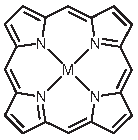
\includegraphics[valign=b]{figures/cpds/porphine.pdf} & 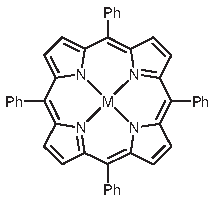
\includegraphics[valign=b]{figures/cpds/tpp.pdf} \\*
    \cmpd{porphine} & \cmpd{tpp} \\   \hline
    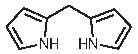
\includegraphics[valign=b]{figures/cpds/dpm.pdf}  & 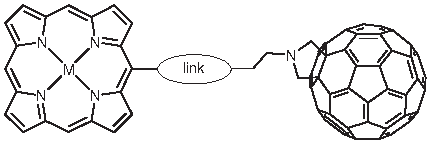
\includegraphics[valign=b]{figures/cpds/dyad.pdf} \\*
    \cmpd{dpm} & \cmpd{dyad} \\ \hline
    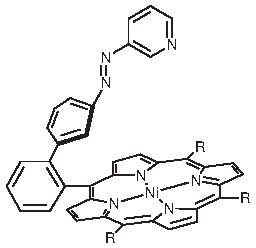
\includegraphics[valign=b]{figures/cpds/switch.pdf} & 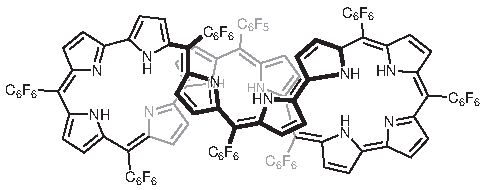
\includegraphics[valign=b]{figures/cpds/osuka52.pdf} \\*
    \cmpd{switch} & \cmpd{osuka52} \\  \hline
    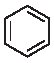
\includegraphics[valign=b]{figures/cpds/benzene.pdf} & 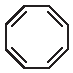
\includegraphics[valign=b]{figures/cpds/cot.pdf} \\*
    \cmpd{benzene} & \cmpd{cot} \\ \hline
    
\includegraphics[valign=b]{figures/cpds/cbd.pdf} & 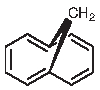
\includegraphics[valign=b]{figures/cpds/tenannulene.pdf} \\*
    \cmpd{cbd} & \cmpd{tenannulene} \\ \hline
    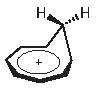
\includegraphics[valign=b]{figures/cpds/homoarom.pdf} & 
\includegraphics[valign=b]{figures/cpds/trishomoarom.pdf} \\*
    \cmpd{homoarom} & \cmpd{trishomoarom} \\  \hline
    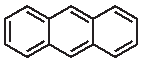
\includegraphics[valign=b]{figures/cpds/anthracene.pdf} & 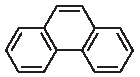
\includegraphics[valign=b]{figures/cpds/phenanthrene.pdf} \\*
    \cmpd{anthracene} & \cmpd{phenanthrene} \\ \hline
    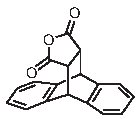
\includegraphics[valign=b]{figures/cpds/anthYes.pdf}  & 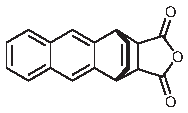
\includegraphics[valign=b]{figures/cpds/anthNo.pdf} \\*
    \cmpd{anthYes} & \cmpd{anthNo} \\ \hline
    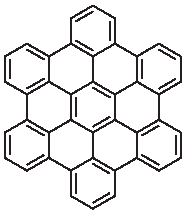
\includegraphics[valign=b]{figures/cpds/HBC.pdf} & 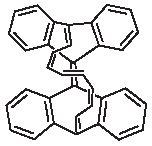
\includegraphics[valign=b]{figures/cpds/herges.pdf} \\*
    \cmpd{HBC} & \cmpd{herges} \\ \hline
    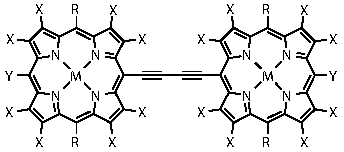
\includegraphics[valign=b]{figures/cpds/p2.pdf} & 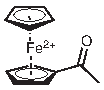
\includegraphics[valign=b]{figures/cpds/monoacfc.pdf} \\*
    \cmpd{p2} & \cmpd{monoacfc} \\ \hline





\end{longtable}
\endgroup
\end{center}
%\end{table}

%\end{multicols}
\end{listofcpds} \mtcaddchapter


%\listoffigures
%	\mtcaddchapter
% \mtcaddchapter is needed when adding a non-chapter (but chapter-like) entity to avoid confusing minitoc

% Uncomment to generate a list of tables:
%\listoftables
%	\mtcaddchapter
\markboth{List of Abbreviations}{List of Abbreviations}
%%%%% LIST OF ABBREVIATIONS
% This example includes a list of abbreviations.  Look at text/abbreviations.tex to see how that file is
% formatted.  The template can handle any kind of list though, so this might be a good place for a
% glossary, etc.
%\include{text/abbreviations}


\newlength{\nomitemorigsep}
\setlength{\nomitemorigsep}{\nomitemsep}
\setlength{\nomitemsep}{-\parsep}


\renewcommand{\nomgroup}[1]{%
\itemsep\nomitemorigsep%
\ifthenelse{\equal{#1}{S}}{\item[\normalsize{\textbf{Symbols}}]}{%
\ifthenelse{\equal{#1}{A}}{\item[\normalsize{\textbf{Abbreviations}}]}{}}%
\itemsep\nomitemsep}
%\setlength{\baselineskip}{0pt} 
%\begin{multicols}{2}
\small{%
\printnomenclature[2.1cm]}
%\end{multicols}
	\mtcaddchapter
% The Roman pages, like the Roman Empire, must come to its inevitable close.
\end{romanpages}

\fi
%%%%% CHAPTERS
% Add or remove any chapters you'd like here, by file name (excluding '.tex'):
\flushbottom


% so that we start counting references for the main text only
\newrefsection

%!TEX root = ../thesis.tex
%!TEX spellcheck
% \begin{savequote}[8cm]
% Neque porro quisquam est qui dolorem ipsum quia dolor sit amet, consectetur, adipisci velit...

% There is no one who loves pain itself, who seeks after it and wants to have it, simply because it is pain...
%   \qauthor{--- Cicero's \textit{de Finibus Bonorum et Malorum}}
% \end{savequote}

\begin{savequote}[8cm]
Reader! Imagine a school-boy who has outgrown his clothes. Imagine the repairs made on the vestments where the enlarged frame had burst the narrow limits of its inclosure. Imagine the additions made where the projecting limbs had fairly and far emerged beyond the confines of the garment. Imagine the boy still growing, and the clothes, mended all over, now more than ever in want of mending -- such is chemistry, and such its nomenclature.
  \qauthor{--- John Joseph Griffin in Chemical Recreations (7th Edition, 1834) ``The Romance of Chemistry'' p. 189}
\end{savequote}

\chapter{\label{ch:intro}Introduction} 

\minitoc

\section{Outline}
		%\nomenclature{h}{Hour}\nomenclature{min}{Minute}\nomenclature{s}{Second}

	This thesis explores electron delocalisation in porphyrin-based molecular wires, in both linear and cyclic topologies, and in neutral, cationic and excited electronic states. There is some necessity for restriction in the content of the introduction, and so only a very limited presentation of porphyrin chemistry will be made. Interested readers are referred to recent reviews,\autocite{Vicente2014,Tanaka2015,Wang2016,Hiroto2016} and to other theses from the Anderson group which deliver comprehensive introductions to porphyrin chemistry.\autocite{KondratiukThesis2013,LiuThesis2016,KamonsutthipaijitThesis2016} The literature surrounding delocalisation of unpaired electrons (\ltt{e.g.} radical cations) on conjugated oligomers and in mixed-valence compounds is mainly dealt with in \autoref{ch:radcat}. For the most part, this introduction will be limited to a discussion of aromaticity, particularly in the context of organic molecules. A brief introduction to computational techniques for the assignment and prediction of aromaticity will be given.

\section{Porphyrins}

	Porphyrins, with their vivid colours, have captured chemists' imaginations since the discovery of the chemical properties of chlorophyll by Willst\"atter, for which he was awarded the Nobel Prize in 1915.\autocite{Willstatter1915,Robinson1953} Chlorophyll, heme, and cytochrome proteins all contain porphyrins, and they all prove vitally important to life.

	The simplest porphyrin is porphine \cmpd{porphine} (\autoref{fig:intro:porphs}), comprising four pyrroles and four methines, arranged to form a tetrapyrrolic macrocycle with an aromatic 18 \pii{}-electron circuit. The 18 \pii{}-electron circuit can be represented by simplifying the porphyrin to an [18]-annulene (shown in red for tetraphenylporphyrin, TPP, \cmpd{tpp} in \autoref{fig:intro:porphs}) or to a [16]-annulene dianion.\autocite{Johnson1971,Vogel1993} The atomic positions of porphine can be identified by the IUPAC\nomenclature{IUPAC}{International Union of Pure and Applied Chemistry} systematic numbering (\cmpd{porphine}) or by the common nomenclature. In the common nomenclature the methines are referred to as the \textit{meso} positions, the pyrrole \ce{C-H}s are referred to as the $\beta$ positions, and the quaternary pyrrole carbons are the $\alpha$ positions, as illustrated on TPP \cmpd{tpp}. 

	Porphyrins are typically synthesised by condensation of an aldehyde and pyrrole, perhaps \ltt{via} a dipyrromethane (\cmpd{dpm}, see for example \autoref{fig:intro:porphs}).\autocite{Littler1999b,Littler1999} The resulting porphyrin monomers can be elaborated by oligomerisation, or by the introduction of substituents. In the former case, discrete porphyrin oligomers in diverse morphologies, with different linker groups, can be readily prepared (see later).\autocite{Tanaka2015,Wang2016} As an example of the latter case, dyads (\ltt{e.g.} \cmpd{dyad}) and triads can be prepared for exploring photoinduced charge separation.\autocite{Guldi2002,Gilbert2015} 

	\begin{figure}[ht!]
		\replacecmpd{porphine}
		\replacecmpd{tpp}
		\replacecmpd{dyad}
		\replacecmpd{dpm}
		\centering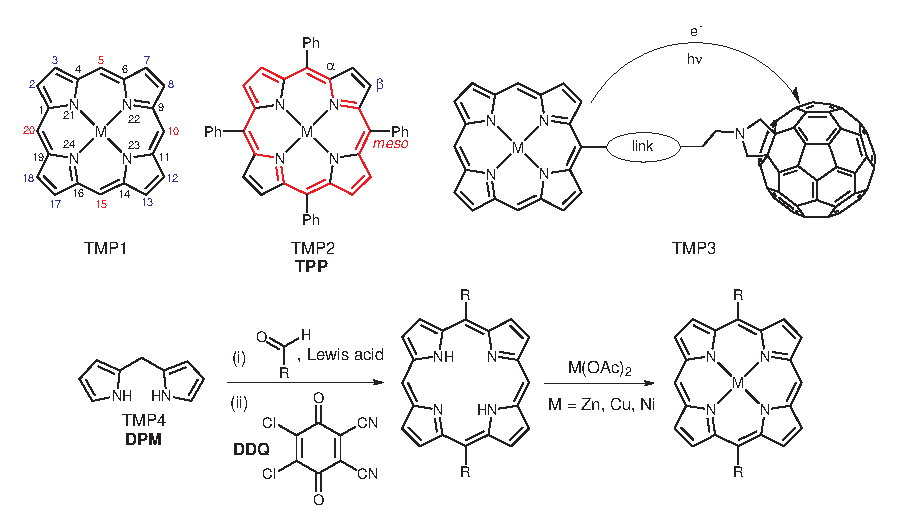
\includegraphics{figures/intro/porphyrin-numbering.eps} 
		\caption[]{(top) Examples of porphyrins: \cmpd{porphine} is porphine, with IUPAC atom numbering indicated; \cmpd{tpp} is tetraphenylporphyrin (TPP), with the [18]-annulene aromatic circuit indicated in red, and with the `common names' for the atomic positions; \cmpd{dyad} is a schematic example of a \ce{C60}--porphyrin dyad, in which absorption of a photon of light can result in charge separation. (bottom) Example of porphyrin synthesis by condensation of an aldehyde with DPM \cmpd{dpm}, followed by oxidation with DDQ\@. Metal insertion then follows.}
		\label{fig:intro:porphs}
	\end{figure}


	The introduction of a central metal ion into a porphyrin, which acts as a square planar tetradentate ligand, allows further modulation of the porphyrin's properties. For example, a nickel(II) porphyrin \cmpd{switch} has been used as a photochemical spin switch, where the action of the azobenzene photoswitch causes an axial pyridine to coordinate to the Ni(II), changing it from low spin ($S=0$) to high spin ($S=1$) (\autoref{fig:intro:switches}).\autocite{Venkataramani2011} Copper(II) porphyrins are paramagnetic; they have been explored for their applications as biochemical distance rulers by double electron-electron resonance (DEER\nomenclature{DEER}{Double electron-electron resonance}).\autocite{Bowen2016} Axial coordination of ligands to metalloporphyrins, yielding square pyramidal or octahedral coordination geometries, is useful for the synthesis of supramolecular assemblies (\autoref{fig:intro:porphy-supra}), as has been recently reviewed.\autocite{Wang2016}

	\begin{figure}[ht!]
		\replacecmpd{switch}
		\centering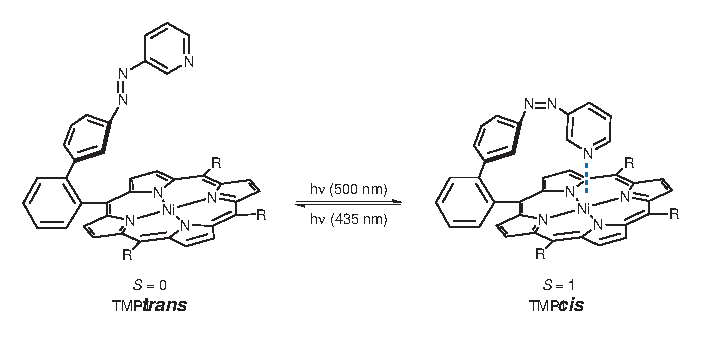
\includegraphics{figures/intro/switch.eps} 
		\caption[]{A photochemically mediated spin switch employing an azobenzene link which, upon irradiation with \SI{500}{\nano\metre} light, undergoes a \textit{trans}--\textit{cis} isomerism, causing a pyridine ligand to axially coordinate the Ni(II) and switching the spin state from low spin (\textit{\textbf{trans}}) to high spin (\textit{\textbf{cis}}).\autocite{Venkataramani2011}}
		\label{fig:intro:switches}
	\end{figure}

	This thesis concerns the chemistry of butadiyne-linked zinc-porphyrin oligomers. This class of oligomer was first prepared by Arnold in 1978,\autocite{Arnold1978} and has since been the subject of intense study, mainly by his group and that of Anderson.\autocite{Arnold1992,Arnold2000,Anderson1994,Anderson1999} Historically, Arnold focused primarily on the physical properties of short oligomers (\ltt{e.g.} porphyrin dimers),\autocite{Arnold2000} whilst Anderson explored the supramolecular chemistry of porphyrins. The Anderson group has prepared spectacular structures such as porphyrin ladders,\autocite{Taylor1999} the nanoring-template complex \rwt6,\autocite{Hoffmann2008} the Vernier-templated figure-of-eight \cp{12}$\bullet{}$\temp{6\tsub2},\autocite{OSullivan2011} ring-in-ring complexes,\autocite{Rousseaux2015} and an axially elongated nanoring tube \tubewt{} (\autoref{fig:intro:porphy-supra}).\autocite{Neuhaus2015} The preparation of these structures has relied on the binding of nitrogenous ligands -- typically pyridine -- to the axial coordination site of the Zn-porphyrin. The Zn-porphyrin--pyridine binding constant is weak ($K = 10^4\ \si{\per\Molar}$),\autocite{Cole1972} but chelate cooperativity diminishes the entropic cost for multiple-binding, leading to huge binding constants.\autocite{Hogben2011} For example, \temp6 in \rwt6 has a binding constant of $K = 10^{36}\ \si{\per\Molar}$.\autocite{Hoffmann2008} The butadiyne link ensures good conjugation between the porphyrin units, which can readily adopt a coplanar conformation without steric hindrance, in contrast to the steric clash between porphyrin $\beta$-protons in a planar monoalkyne-linked dimer. However, as we will see in \autoref{ch:dimer}, there is little thermodynamic preference for planarity: the barrier to torsional rotation in a butadiyne-linked porphyrin dimer is about \SI{2}{\kilo\joule\per\mole}.\autocite{Winters2007,Peeks2016} As such, butadiyne-linked porphyrin oligomers are prone to the introduction of conjugation-breaking defects in the form of non-planarity of adjacent porphyrin units. 


	\begin{figure}[ht!]
		\centering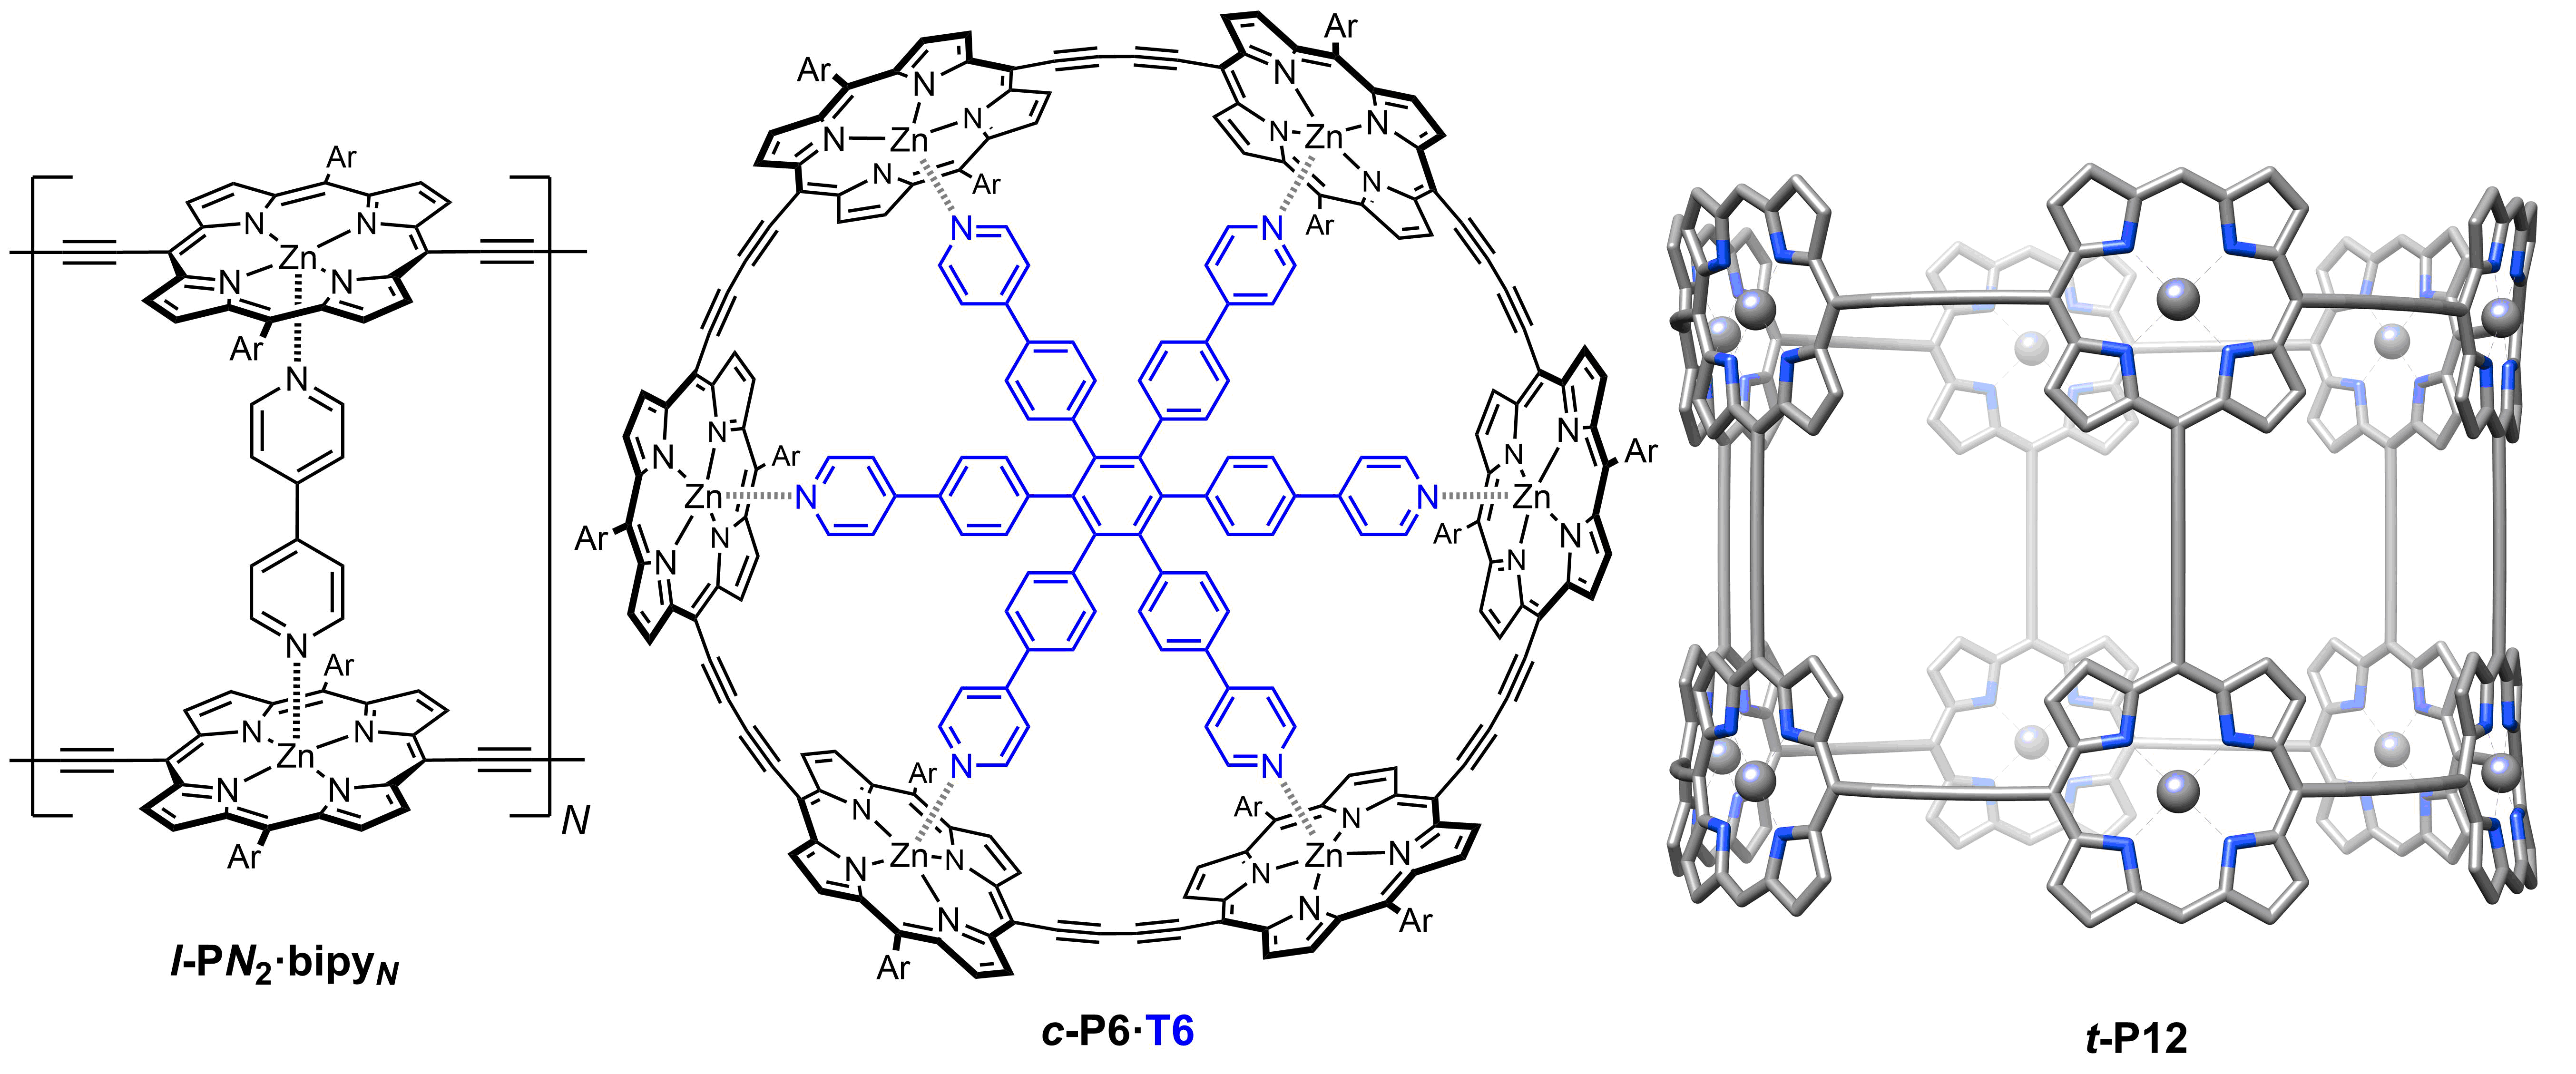
\includegraphics[width=\textwidth]{figures/intro/porphy-supra.png} 
		\caption[]{A double-stranded porphyrin ladder formed by coordination of 4,4\tsup{\textprime{}}-bipyridine (bipy\nomenclature{bipy}{4,4\tsup{\textprime{}}-Bipyridine}),\autocite{Taylor1999} a [6]-porphyrin nanoring \rwt6,\autocite{Hoffmann2008} and a [12]-porphyrin nanotube (BLYP/6-31G*) \tp{12}.\autocite{Neuhaus2015}}
		\label{fig:intro:porphy-supra}
	\end{figure}


	\begin{figure}[ht!]
		\centering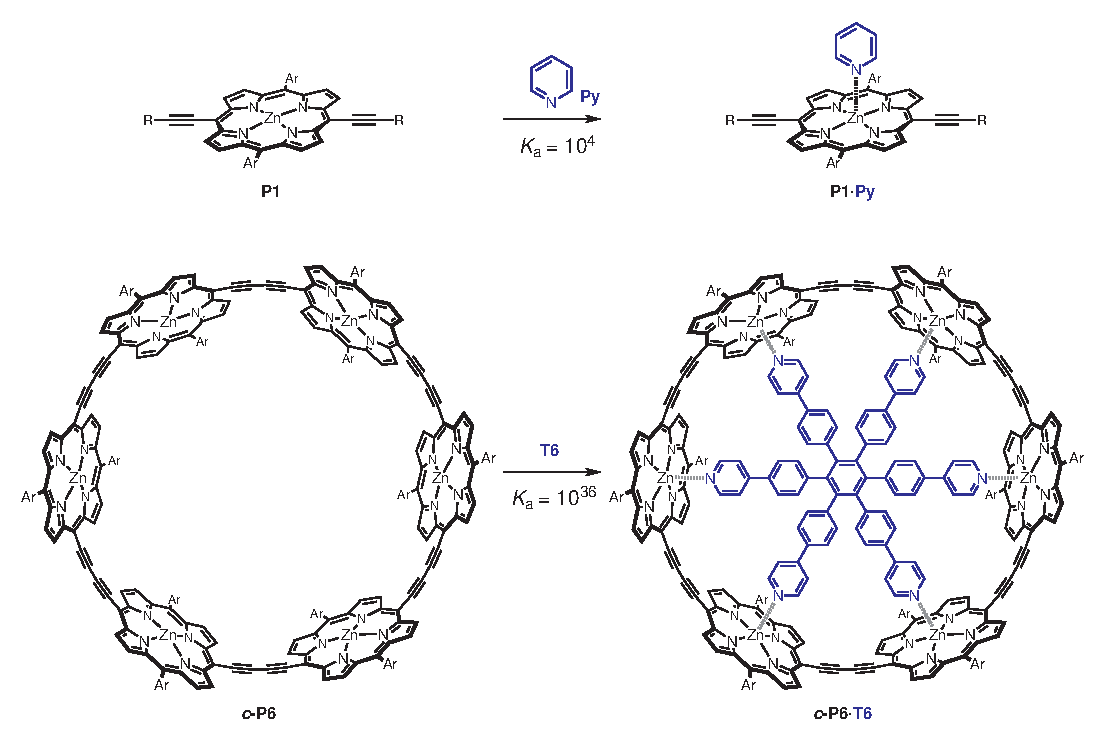
\includegraphics[width=\textwidth]{figures/intro/porphy-binding.eps} 
		\caption[]{Comparison of binding constants for a porphyrin monomer to pyridine and for a [6]-porphyrin nanoring \cp6 to a hexadentate template \temp6, demonstrating significant cooperativity in the latter.}
		\label{fig:intro:porphy-binding}
	\end{figure}



	The high absorption coefficients of porphyrins and their oligomers often motivate comparisons to the light harvesting complexes in green plants, which comprise circular arrays of chlorophyll molecules.\autocite{VanGrondelle1994,McDermott1995} Efforts continue to use porphyrins in high-efficiency dye-sensitised solar cells (DSSCs)\nomenclature{DSSC}{Dye-sensitised solar cell}, through both the design of new materials and investigations into electron transport properties.\autocite{Higashino2015,Gilbert2015} To date, the power conversion efficiency of synthetic DSSCs has reached 12\%, compared to 22\% for leading perovskite materials and 26\% for silicon cells.\autocite{NREL2016} The theoretical limit for a single-junction cell, the Shockley-Queisser limit, is 34\%.\autocite{Shockley1961} Porphyrins have found more application in medicine, where they are employed for photodynamic therapy (PDT\nomenclature{PDT}{Photodynamic therapy}). In this treatment for cancer, a sensitiser molecule (porphyrin) accumulates in a tumour and is then irradiated with light. Intersystem crossing to the triplet manifold occurs, resulting in sensitisation of oxygen and oxidative destruction of tissue.\autocite{Mody2000,Ethirajan2011}

	The field of porphyrin chemistry is broadened by the introduction of the porphyrinoids and the expanded and contracted porphyrins.\autocite{Stepien2011,Mack2016} These molecules are essentially variations upon the theme of the porphyrin: for example, diverse porphyrinoids can be generated by replacing the pyrroles of the macrocycle with other 5-membered aromatic rings, like furan or thiophene.\autocite{Vogel1989,Vogel2000} Expanded porphyrins (\ltt{e.g.} \cmpd{osuka52}, \autoref{fig:intro:osuka}) are simply large porphyrinoids, with at least 17 atoms in their `internal ring pathway'.\autocite{Sessler2003,Saito2011} The diversity of porphyrinoids has proven extremely useful for dissecting concepts in aromaticity,\autocite{Osuka2011,Stepien2011,Wu2013,Pawlicki2015} including excited state and M\"obius aromaticity, as we shall see in the next section. 

	\begin{figure}[ht!]
		\replacecmpd{osuka52}
		\centering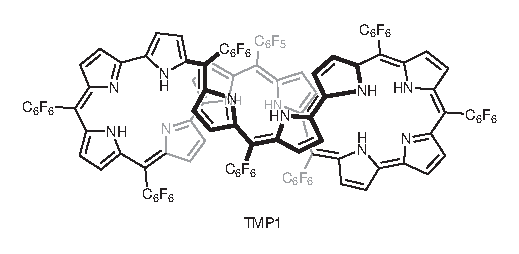
\includegraphics{figures/intro/osuka.eps} 
		\caption[]{Osuka's H\"uckel aromatic [50]-\pii{} expanded porphyrin \cmpd{osuka52}.\autocite{Soya2015}}
		\label{fig:intro:osuka}
	\end{figure}

\FloatBarrier

\section{Aromaticity}
	Aromaticity is a heavily-reviewed topic, and was the subject of entire issues of \textit{Chem. Rev.} in 2001 and 2005,\autocite{Schleyer2001,Schleyer2005} and of \textit{Chem. Soc. Rev.} in 2015.\autocite{Martin2015} In this section, a brief historical account of aromaticity will be given, illustrated by prominent examples. 

	A simple bibliometric analysis using Google Books\autocite{Michel2011} shows that, although benzene was widely written about from the late 1800s, the concept of `aromaticity' only gained prominence with the appearance of molecular orbital theory, ring current theories, and NMR (\autoref{fig:intro:ngram}a, nuclear magnetic resonance). This correlation describes the development of aromatic chemistry, from the study of compounds with particular olfactory properties to the broad-ranging subject of aromaticity, facilitated by synthetic, spectroscopic, and computational advances. 

		\begin{figure}[ht!]
			\centering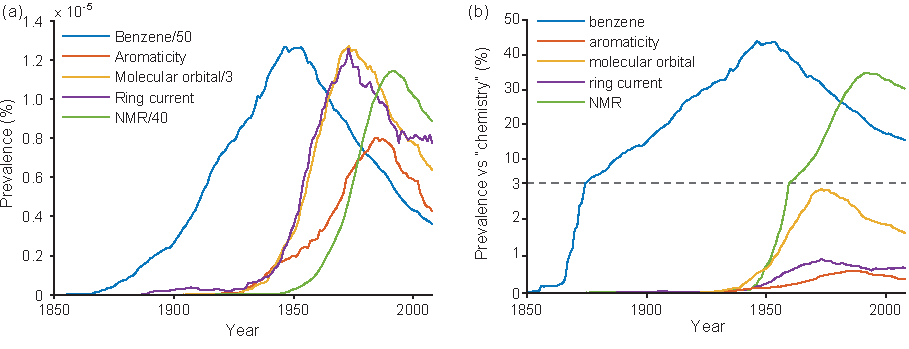
\includegraphics{figures/intro/ngram.pdf} 
			\caption[]{Bibliometric analysis (ngrams)\autocite{Michel2011} showing the use of benzene, aromaticity, molecular orbital, ring current and NMR in the English language corpus of Google Books.\autocite{Michel2011} In (a) the prevalence of each phrase, case insensitive, is shown. The numbers in the legends denote a scale factor applied to the specified term. In (b) the prevalence of the (case sensitive) terms relative to the prevalence of the word `chemistry' are shown. All data are smoothed with a 10-point (21-year) moving average.}
			\label{fig:intro:ngram}
		\end{figure}

	The decline in frequency in all of these terms since the mid-1900s is partly a consequence of chemistry forming a smaller part of the English language corpus in modern times. In \autoref{fig:intro:ngram}b, the frequencies of several terms relating to aromaticity are normalised by the frequency of the word `chemistry'. The results show that relative to chemistry, interest in ring currents and aromaticity has remained fairly steady since the 1980s. It is reflective of benzene's importance that in the 1940s, the word `benzene' was mentioned almost half as many times as the word `chemistry'!

	\subsection{Early aromaticity}

		Benzene (\cmpd{benzene}, \autoref{fig:intro:aromatics}) was isolated by Faraday in 1825, but its structure remained unknown until the 1860s. After Kekul\'e and Coupers' independent realisations that carbon is tetravalent,\autocite{Kekule1858,couper1858nouvelle} the former deduced (through the famous, perhaps apocryphal, day-dream of a snake biting its own tail) that benzene is cyclic.\autocite{kekule1865constitution} Kekul\'e proposed a benzene structure with alternating single and double bonds, which he later refined by the suggestion that the single and double bonds rapidly interconverted.\autocite{kekule1866untersuchungen} Benzene and the other aromatic molecules became defined by reactivity, most notably by the fact that they underwent a substitution reaction with bromine, as opposed to the addition expected for alkenes (\autoref{fig:intro:arom-rx}). 

		\begin{figure}[ht!]
			\replacecmpd{benzene}
			\replacecmpd{cot}
			\replacecmpd{cbd} 
			\replacecmpd{tenannulene}
			\replacecmpd{homoarom}
			\replacecmpd{trishomoarom}
			\centering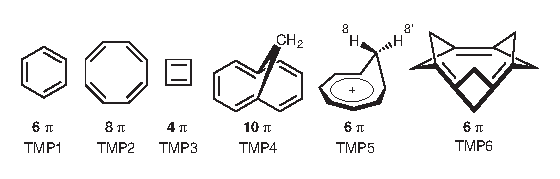
\includegraphics{figures/intro/aromatics.eps} 
			\caption[]{Examples of aromatic, non-aromatic, and antiaromatic compounds.}
			\label{fig:intro:aromatics}
		\end{figure}

		\begin{figure}[ht!]
			\centering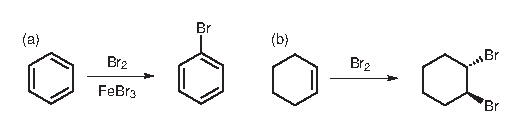
\includegraphics{figures/intro/arom-rx.eps} 
			\caption[]{(a) Benzene undergoes a substitution reaction with bromine, in the presence of \ce{FeBr3} as an activating Lewis Acid; (b) cyclohexene undergoes an addition reaction with benzene.}
			\label{fig:intro:arom-rx}
		\end{figure}

		Thiele proposed a theory to account for this reactivity, namely that unsaturated carbons had a `partial valence', which was especially reactive.\autocite{Thiele1899} Adjacent pairs of partial valences could interact with (saturate) each other, provided neither was at a terminal position (hence, the partial valences in ethylene could not saturate). Reactivity was thus found at the unsaturated partial valences, explaining the reactivity at the 1,4-positions of 1,3-butadiene and the stability of benzene (\autoref{fig:intro:thiele}). However, Thiele's theory was proven wrong by our earlier hero of chlorophyll chemistry, Willst\"atter, who isolated cyclooctatetraene (COT\nomenclature{COT}{Cyclooctatetraene}, \cmpd{cot}) in 1911,\autocite{Willstatter1911} and found that it reacted with bromine as an alkene, without any hint of partial valence stabilisation.

		\begin{figure}[ht!]
			\centering
\includegraphics{figures/intro/thiele-valence.eps} 
			\caption[]{Thiele's theory of partial valences applied to (a) ethylene, (b) 1,3-butadiene and (c) benzene. Partial valences are indicated by dotted lines: blue dotted lines are unsatisfied partial valences, and thus sites of high reactivity. Saturated partial valences are denoted by red dotted semicircles: these positions are unreactive.}
			\label{fig:intro:thiele}
		\end{figure}

		Although much research into aromatic compounds continued in the latter part of the 19\nth century, heavily motivated by their application in dyestuffs, the notion of aromaticity as a distinct chemical property did not really exist until the 1930s, with the development of molecular orbital theory, and only became ascendant as late as the 1950s (\autoref{fig:intro:ngram}). %Amusingly, a statement by Gilman and Towne on (super-)aromaticity in 1932 would not be out of place in a review published today:\autocite{Gilman1932}

		%\begin{quote}
		%	Aromatic properties are the peculiar properties exhibited by aromatic compounds. Actually, there is no agreement as to what constitutes aromatic compounds or aromatic properties. We do not know exactly what peculiarities in unsaturation are necessary to give a cyclic compound aromatic properties. Nor is there concordance of opinion as to the particular properties which are characteristic of aromatic compounds.
		%\end{quote}

	\subsection{The aromatic sextet and H\"uckel's theory}

		Crocker, Armit and Robinson presented the idea of the \textit{aromatic sextet} in the 1920s, proposing that benzene's aromatic stability arose from the favourability of a sextet of valence electrons.\autocite{Crocker1922,Armit1925,Balaban2005} Pauling and Wheland soon developed valence bond (VB) theory and the accompanying notion of resonance was quickly adopted by organic chemists. Benzene's aromatic stabilisation was explained by the presence of multiple resonance structures, in which the delocalised \pii{}-electrons are represented by different VB representations: more resonance structures confer more stability.\autocite{pauling1933nature} Although Erich H\"uckel's molecular orbital (MO) theory was developed in the 1930s, and was able to quantitatively explain the stability of aromatic molecules, his explanations struggled to displace the pervasive and simple resonance theory.\autocite{huckel1937grundzuge,berson1999chemical} It was really only with the development of mnemonics, such as Doering's presentation of the $[4n+2]$ rule\autocite{Doering1951} (bringing the theory back to aromatic sextets) and Frost and Musulin's graphical presentation of H\"uckel's orbital energies\autocite{Frost1953} that H\"uckel's MO theory entered the mainstream.\autocite{berson1999chemical} The familiar $[4n+2]$ rule states that a molecule with $[4n+2]$ conjugated \pii{}-electrons is aromatic, while a molecule with $[4n]$ \pii{}-electrons is antiaromatic, where $n$ is a non-negative integer. 

		By constructing the Frost-Musulin diagrams for benzene and cyclobutadiene (CBD\nomenclature{CBD}{Cyclobutadiene}, antiaromatic, \cmpd{cbd})  we can immediately see that benzene, in a \symm{D}{6h} model, has a filled degenerate pair of orbitals as its highest-occupied MO (HOMO), whereas CBD, with only $[4n]$ \pii{}-electrons, adopts a triplet configuration in its \symm{D}{4h} symmetric structure (\autoref{fig:intro:huckel}). Further calculations reveal that CBD is better described as a \symm{D}{2h} rectangle, with increased double-bond and single-bond character (\ltt{i.e.} bond length alternation, BLA) compared to benzene.\autocite{Bally1980} This pseudo-Jahn-Teller (PJT\nomenclature{PJT}{Pseudo-Jahn-Teller})\autocite{Kertesz2005} distortion is common to the $[4n]$-\pii{} antiaromatic molecules, and lifts the HOMO degeneracy as shown in \autoref{fig:intro:huckel}, leading to a closed shell antiaromatic configuration with a small HOMO--LUMO (lowest unoccupied MO) gap.

		\begin{figure}[ht!]
			\centering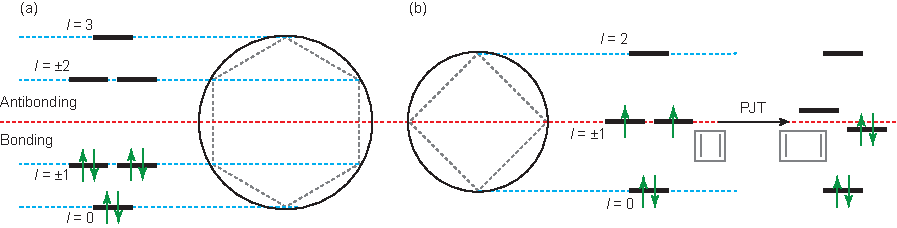
\includegraphics{figures/intro/huckel.pdf} 
			\caption[]{Frost-Musulin diagrams for (a) benzene and (b) CBD\@. In (a), all of the bonding orbitals (below the horizontal red line) of benzene are filled. In (b), the half-occupied degenerate pair is non-bonding. A pseudo-Jahn-Teller (PJT) distortion breaks the degeneracy and leads to a bonding character for one electron pair.}
			\label{fig:intro:huckel}
		\end{figure}

		\FloatBarrier

	\subsection{Ring currents}

		In addition to advances in theory, the early part of the 20\nth century saw a development of experimental methods for the quantification of aromaticity. Pascal noted that aromatic molecules were more diamagnetic ($\chi_\text{M}$) than expected on the basis of additive substituent contributions ($\chi_{\text{M}}^\prime{}$),\autocite{pascal1910magnetochemical} and Pacault termed this excess of diamagnetic susceptibility the `exaltation' ($\Lambda$).\autocite{Pacault1961,Gleiter2012} 

		\begin{equation}
			\Lambda = \chi_\text{M} - \chi_{\text{M}}^\prime{}
		\end{equation}

		The utility of exaltation measurements for the assignment of aromaticity was demonstrated by Dauben \ltt{et al.} in 1969,\autocite{Dauben1969} but by this time there was a more experimentally informative, and appealing, method of measuring magnetic properties: NMR\@. Nowadays, susceptibility measurements have almost entirely fallen out of favour,\autocite{Gershoni-Poranne2015} despite the fact that they were once described as the `only' unambiguous assignor of aromaticity.\autocite{Schleyer1996a}

		NMR is a particularly helpful descriptor of aromaticity because of the effect of so-called aromatic ring-currents on NMR chemical shifts. The resonances of nuclei inside an aromatic ring are shielded; those outside are deshielded. For example, the protons of benzene are deshielded from an olefinic chemical shift (5~ppm)\nomenclature{ppm}{Parts per million} to what is now colloquially called `the aromatic region', around 7~ppm. In the ring-current model (RCM)\nomenclature{RCM}{Ring-current model} the delocalised \pii{}-electrons in an aromatic ring precess about the ring centre in the presence of an external magnetic field $B_\text{ext}$ (typically defined along the $z$ axis, perpendicular to the molecular plane). This precession is a \textit{diatropic} current of electrons which flows clockwise around the ring, when viewed from the $z$ axis (looking towards $-z$) (\autoref{fig:intro:ringcurr}). Consistent with Amp\`ere's right hand screw rule, this induced ring-current $J_\text{ind}$ has an associated magnetic field $B_\text{ind}$, which opposes $B_\text{ext}$ inside the ring (hence has a shielding effect) and reinforces $B_\text{ext}$ outside the ring (hence deshielding). Examples of the shielding and deshielding effects arising from the RCM will be discussed shortly, but first we must give a surprisingly late introduction to antiaromaticity, via the annulenes.

		\begin{figure}[ht!]
			\centering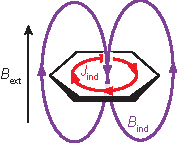
\includegraphics{figures/intro/ring-current.pdf} 
			\caption[]{Representation of the induced ring current ($J_\text{ind}$) in benzene in the presence of an applied magnetic field  ($B_\text{ext}$). The induced current generates its own magnetic field, $B_\text{ind}$ which opposes $B_\text{ext}$ inside the ring, and reinforces it outside.}
			\label{fig:intro:ringcurr}
		\end{figure}

		Benzene, COT and CBD are all members of the class of molecules termed the \textit{annulenes} by Sondheimer.\autocite{Sondheimer1962} Annulenes are ring systems of general formula C\tsub{\textit{m}}H\tsub{\textit{m}} comprising alternating single and double C--C bonds. Sondheimer prepared a spectacular array of annulenes and dehydroannulenes, in which some \ce{C=C} bonds are replaced with \ce{C#C} bonds.\autocite{Sondheimer1963,Sondheimer1967,Sondheimer1972} He made the remarkable discovery that while the $[4n+2]$-annulenes exhibited NMR spectra similar to that of benzene: \ltt{i.e.} shielded inner resonances and deshielded outer resonances, the $[4n]$-annulenes had reversed spectra: inner resonances were deshielded and outer resonances shielded.\autocite{Sondheimer1967} 

		The term \textit{antiaromatic} was first applied by Breslow in 1965 to describe the instability exhibited by some molecules with $[4n]$ \pii{}-electrons, antithetical to the established aromatic stabilisation of $[4n+2]$-\pii{} molecules.\autocite{Breslow1965} In antiaromatic molecules, the ring current flows in the opposite direction (\textit{paratropic}) to that in aromatic molecules,\autocite{Steiner2001} which accounts for the opposite effects on chemical shifts.

		It is important to note that both aromatic and antiaromatic molecules simultaneously possess counter-rotating diatropic and paratropic ring current character to different extents. The diatropic ring current (and the diamagnetic susceptibility) is a ground state property; paratropic currents (and temperature-independent paramagnetic susceptibility) arise from interactions with excited states.\autocite{Longuet-Higgins1967} It is easy to see why the paratropic currents can dominate for antiaromatic molecules due to the smaller HOMO-LUMO gap. 

		In a H\"uckel theory approximation, a symmetric annulene has a manifold of \pii{}-orbitals with angular momentum values $l = 0, \pm{}1, \pm{}2 \mathellipsis{}$. For aromatic molecules with $[4n+2]$ \pii{}-electrons, these orbitals are filled to $l=\pm n$. In the antiaromatic case, the degenerate pair $l=\pm n$ is only half-filled, and can undergo distortions to lift the $l=\pm n$ degeneracy and afford a HOMO with $l = n$ and LUMO with $l = -n$. The HOMO--LUMO gap is small in this case, compared to that for an aromatic molecule (\autoref{fig:intro:huckel}), so the excited state transition (and accompanying change in angular momentum) which induces the paratropic ring currents is more accessible.\autocite{Longuet-Higgins1967,Pople1966} 

		Fowler and Steiner have presented an alternative model in which the ring current direction is predicted by the symmetry of the dominant frontier-orbital transitions -- in this model, both diatropic and paratropic ring currents arise from transitions to excited states. A rotationally allowed transition (as between a Jahn-Teller distorted angular-momentum pair) leads to a paratropic current, while a translationally allowed transition (as between $l=\pm{}n$ and $l=\pm [n+1]$) leads to diatropicity.\autocite{Fowler2001,Steiner2001} More thorough introductions to the quantum mechanical origin of ring currents and magnetic susceptibilities can be found in the cited reviews and references therein.\autocite{Lazzeretti2000,Gomes2001}

	 	The NMR shielding effect inside an aromatic ring can be probed by molecules where an NMR-active nucleus is located inside the ring. Vogel and coworkers were able to synthesise a [10]-annulene derivative with a methylene bridge above the annulene plane (1,6-methanocyclodecapentaene, \cmpd{tenannulene}): as expected from the RCM, this methylene is shielded by about \SIrange{2}{3}{\ppm} to \SI{-0.5}{\ppm}.\autocite{Vogel1967} The propensity of \ce{Li+} to coordinate to the \pii{}-systems of aromatic molecules can also be exploited, allowing the use of \nmriso{7}{Li} NMR to measure the ring-current shielding effect.\autocite{Schleyer1996a}

	 	Porphyrin chemistry provides many examples of the ring current shielding effects for aromatic and antiaromatic derivatives. The porphine ligand is formally in a $2-$ oxidation state with an aromatic set of $18$ \pii{}-electrons. Typically, a $2+$ metal binds to the porphyrin to give a net zero charge, as is the case for M = Zn, Mg, Ni, 2H, \ltt{etc}. In the latter case, M = 2H, the protons are characteristically shielded from a pyrrolic \SI{8}{\ppm} to \SI{-2}{\ppm}. Vaid and coworkers have prepared a TPP complex of Si, where the TPP ligand has a $-4$ ($20\pi$) oxidation state. \nmriso{29}{Si} NMR shows that the central Si is deshielded by \SI{125}{\ppm} on account of the antiaromatic ring-current.\autocite{Cissell2005}

	\subsection{Other experimental signs of aromaticity}
		
		There are other properties available by which to assign aromaticity. The most traditional of these is based on aromatic reactivity: a propensity to undergo electrophilic aromatic substitution rather than addition. A related aspect is the energetic stability of aromatic systems, arising from a large resonance stabilisation energy (contrast to zero, or negative, stabilisation for antiaromatic systems). Finally, structural properties can support an assignment of aromaticity: aromatic compounds exhibit a low BLA, whereas the pseudo-Jahn-Teller distortion for antiaromatic compounds leads to a higher BLA\@. Such data can come from infra-red (IR) or Raman spectroscopies, X-ray diffraction, or from calculation.% In the case of benzene, its planar hexagonal structure was confirmed by crystallography of hexamethylbenzene reported by Lonsdale in 1929.\autocite{Lonsdale1929}

	\subsection{Predicting aromaticity}

		There is a multitude of methods available to computationally predict and characterise aromaticity in molecules. Their utility is facilitated by the availability of computing power and the applicability of density functional theory (DFT), which scales well for small molecules (systems with a few hundred atoms are routine) with generally accurate results.



		\subsubsection{Ring currents}\label{sec:intro:rc}

			Perhaps the most popular methods for predicting aromaticity are those which measure the properties of the aromatic ring current. The first of these techniques was the nucleus independent chemical shift (NICS), which evaluates the NMR shielding at a point in space around a molecule. This is achieved by placing a `ghost' atom (in Gaussian, `Bq', after the character (latterly a ghost) Banquo\autocite{shakespeare1903macbeth} in \textit{Macbeth}) at the desired probe position(s). In the first reported NICS calculations, the ghost atoms were placed at the geometric centres of rings.\autocite{Schleyer1996} For some inorganic ring systems, it was noted that the in-plane NICS was prone to contamination by $\sigma$ and in-plane \pii bonds, motivating the dissection of \pii and $\sigma$ components to give NICS\tsub{\pii} and NICS\tsub{$\sigma$}.\autocite{Schleyer1997} The measurement of NICS($X$) at some position $X$ \si{\angstrom} above the ring plane was also used for these inorganic systems, to avoid in-plane contributions.\autocite{Schleyer1997} Indeed, it had been earlier noted that NICS values were higher above the ring plane than in the plane for small \pii{}-aromatic systems, reflecting the toroidal distribution of \pii{}-electrons and the presence of $\sigma$ bond anisotropy contamination for in-plane measurements.\autocite{Schleyer1996} 

			In addition to choosing a suitable $z$-axis height, the selection of the correct tensor component to describe aromaticity is also important: the original report used the isotropic (iso) shielding (NICS\tsub{iso}),\autocite{Schleyer1996} but later studies have placed increased emphasis on the $zz$ shielding tensor component (NICS\tsub{$zz$}) as being more reflective of aromaticity effects. Of the myriad combinations of `dissected NICS' (\ltt{i.e.} \pii contributions only), distances above the ring plane, and tensor components, it was found that NICS(0)\tsub{$\pi zz$} gave the best correlation to aromatic stabilisation energy, and that the non-dissected NICS(1)\tsub{$zz$} was a suitable alternative, since shifting the ghost atom \SI{1}{\angstrom} above the ring plane has the effect of removing most in-plane contamination.

			Since its invention in the late 1990s the NICS method has been extended to the calculation of shielding isosurfaces\autocite{Klod2001} and NICS-scans\autocite{Gershoni-Poranne2014} which reveal the variation in aromaticity in different parts of a molecule.\autocite{Stanger2006,Gershoni-Poranne2014} Examples of the utility of NICS and its derivatives have been thoroughly reviewed.\autocite{Chen2005,Gershoni-Poranne2015} 

			NICS evaluates the effects of the ring current: the magnetic shielding and deshielding. It is also possible to computationally predict and visualise the ring current. The anisotropy of the induced current density (ACID) method depicts the induced current as an isosurface around the molecule.\autocite{Herges2001} By examining this anisotropy property, rather than just the current density field, it is possible to subtract out local diamagnetic (isotropic) atomic ring currents, which otherwise dominate. As a result, electron delocalisation can be visualised as a three-dimensional isosurface around the molecule (\autoref{fig:intro:acid}).

			\begin{figure}[ht!]
				\centering\includegraphics{figures/intro/acid.pdf} 
				\caption[]{ACID isosurfaces (yellow, isovalue = 0.05) and current vectors (green/red) for (a) benzene and (b) a zinc porphyrin monomer. The monomer is substituted with trimethylsilylacetylenes. B3LYP/6-31G* (LANL2DZ ECP for Zn). The current vectors are calculated for an applied magnetic field perpendicular to the aromatic ring planes (\ltt{i.e.} out of the page).}
				\label{fig:intro:acid}
			\end{figure}


			ACID was first applied by Wallenborn \ltt{et al.} to assess transition state aromaticity,\autocite{Wallenborn1998} and the utility of the technique was significantly broadened from aromaticity to other examples of conjugation, including hyperconjugation and spiroconjugation, by Herges \ltt{et al}.\autocite{Herges2001,Geuenich2005} An illustrative example of ACID's application to porphyrin ring currents shows the utility of the technique in dissecting electron delocalisation pathways.\autocite{Wu2013} The additional calculation of induced current vectors shows the direction of electron flow in the presence of an applied field, and thus the assignment of diatropic and paratropic ring currents.\autocite{Geuenich2005}

			It is also possible to directly calculate the magnitude of the ring current passing through a given bond. The Gauge-Including Magnetically Induced Currents (GIMIC) technique is popular for this calculation, and several examples of its use have been reported.\autocite{GIMIC2004,Fliegl2009,Fliegl2012}


		
		\subsubsection{Structural}

			In benzene, all of the \ce{C-C} bonds are of equal length: there is no BLA, indicating complete electron delocalisation. The extent of BLA in a molecule can be quantified using the harmonic oscillator model of aromaticity (HOMA\nomenclature{HOMA}{Harmonic oscillator model of aromaticity})\autocite{Kruszewski1972}

			\begin{align}
				\text{HOMA} &= 1 - \left[\frac{\alpha}{N} \sum_i^N ( R_\text{opt} - R_\text{i})^2\right] \\
				&= 1 - \alpha (R_\text{opt} - R_\text{av})^2 - \frac{\alpha}{N} \sum_i^N( R_\text{av} - R_\text{i})^2 \\
				&= 1 - \text{EN} - \text{GEO}
			\end{align}

			\noindent{}where HOMA is a quantity from 0 (complete localisation) to 1 (complete delocalisation), $\alpha$ is an empirical scaling constant, $N$ is the number of bonds over which the sums run, $R_\text{i}$ is the length of the i\nth bond, $R_\text{av}$ is the average bond length, and $R_\text{opt}$ is the optimum bond length for a fully delocalised bond (\ltt{e.g.} \SI{1.388}{\angstrom} for \ce{C-C}).\autocite{Kruszewski1972} In other words, the first term (EN) relates to an increase (\ltt{vs.} the optimum) in mean bond length in the system, and the second term (GEO) relates to the amount of BLA\@. Both of these parameters indicate non-aromaticity, and hence a decrease in HOMA towards zero.\autocite{Krygowski2000a}

			The theory and application of structural descriptors of aromaticity have been reviewed by Krysowski and Cyra\'nski.\autocite{Krygowski2001} Although BLA is a good metric for aromaticity in small molecules, it has been shown computationally that [30]-annulene exhibits the magnetic characteristics of aromaticity despite the presence of significant BLA, and even larger annulenes (up to [66]-annulene) are aromatic if high symmetry (\symm{D}{6h}) is retained.\autocite{Wannere2003,Choi1998}

		\subsubsection{Energetic}

			The increased thermodynamic stability conferred by aromaticity is often termed the aromatic stabilisation energy (ASE), and can be calculated explicitly. The forerunners of the ASE methods were estimations of resonance energy, either by experiment or calculation.\autocite{Gleiter2012,Cyranski2005}

			In calculations of resonance energy, the additional stabilisation of aromaticity is taken as the difference between the aromatic molecule's energy and the energies of the substituent `localised' components. For example, the resonance energy of benzene can be estimated by the difference of benzene's electron energy and the sum of its bond contributions: three \ce{C=C}, three \ce{C-C} and six \ce{C-H}. These approaches require the energy of the aromatic molecule, and reliable energies for the localised substituents.

			The calculation of ASE depends on devising, and calculating, a suitable reaction scheme which directly reports on the aromaticity of the molecule, whilst avoiding contributions to the reaction energy from changes in hybridisation or atom numbers. The two primary methods are the homodesmotic stabilisation energy (HSE) and its improved form: the isomerisation stabilisation energy (ISE) (\autoref{fig:intro:ase}).\autocite{Schleyer2002} In the former, starting materials and products have the same number of atoms with the same hybridisation. In the latter, the aromatic molecule is optimised with a methyl substituent: the ISE comes from the difference in energy when the methyl is converted into an exocyclic double bond with accompanying loss of aromaticity.

			\begin{figure}[ht!]
				\centering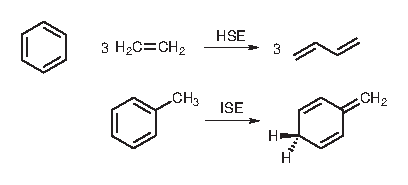
\includegraphics{figures/intro/ase.eps} 
				\caption[]{(top) A homodesmotic reaction for calculating the HSE of benzene; (bottom) the reaction scheme for calculating the ISE of benzene.}
				\label{fig:intro:ase}
			\end{figure}


			The ISE has been evaluated for the annulenes from benzene ([6]-annulene) to [66]-annulene (\autoref{fig:intro:isevspielec}).\autocite{Wannere2003} As ring size increases, ISE-per-electron becomes vanishingly small: for example, [42]-annulene has an ISE-per-electron of \SI{2.3}{\kilo\joule\per\mole}. Put into context, this is about the same as the entropic cost, at room temperature, of freezing a sp\tsup2--sp\tsup2 torsion.\autocite{Mammen1998} This comparison implies that, for large annulenes, the aromatic stabilisation energy becomes vanishingly small compared to the entropic cost of maintaining a regular cyclic geometry necessary for aromaticity.

			\begin{figure}[ht!]
				\centering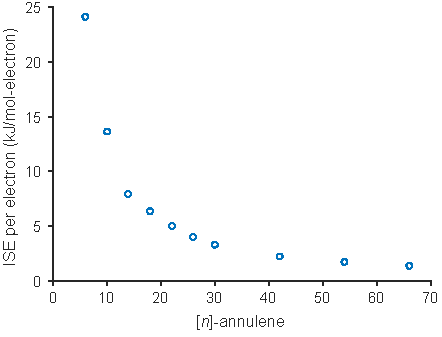
\includegraphics{figures/intro/ise-vs-pielec.pdf} 
				\caption[]{Isomerisation stabilisation energy (ISE) per electron for the annulenes, B3LYP/6-31G*. Data from Wannere and Schleyer.\autocite{Wannere2003}}
				\label{fig:intro:isevspielec}
			\end{figure}



		\subsubsection{Electronic}

			There has been a recent adoption of computational aromaticity metrics which describe electron delocalisation directly, rather than a physical observable such as BLA, or magnetic properties. These metrics have recently been reviewed.\autocite{Feixas2015} Indeed, the ACID method (see Section \ref{sec:intro:rc}) also falls into this category. Without going into too much detail, many electron-delocalisation measures are calculated by evaluating the nature of the electron density at bond critical points and ring critical points (\ltt{i.e.} at the centres of bonds and rings), within the framework of the Quantum Theory of Atoms in Molecules.\autocite{Palusiak2007} In contrast to the other methods presented above, wavefunction analysis is perhaps the most remote from an experimental observable (\ltt{cf.} NMR for NICS, crystallography for structural properties, and calorimetry for stabilisation energies).


	\subsection{Topological effects on aromaticity}

		The annulenes are all monocyclic carbocycles, but molecules can exhibit much broader topological diversity, which has implications for the assignment of aromaticity. In this section we discuss, roughly in order of their appearance in the literature, polycyclic aromaticity and Clar's rule, homoaromaticity, and M\"obius aromaticity.

		\subsubsection{Polycyclic aromaticity}

			Some of the earliest identified aromatic compounds, on the basis of smell, were those comprising fused benzene rings. These molecules exhibit some non-aromatic character in their reactivity: anthracene (\cmpd{anthracene}), comprising three linearly fused benzene rings, undergoes Diels-Alder reaction at the 9,10-positions of the central benzene ring. Phenanthrene (\cmpd{phenanthrene}) has distinctly olefinic chemistry at its 9,10-positions. These observations were rationalised by Clar, who noted that the aromaticity of a polybenzenoid molecule depends on the number, and location, of discrete aromatic sextets of six \pii{}-electrons.\autocite{clar1972aromatic} In anthracene, three resonance structures, each with one sextet, can be drawn; Diels-Alder chemistry at the 9,10-positions offers a product with two Clar sextets (\cmpd{anthYes}), while reaction at either of the terminal benzene rings gives just one Clar sextet (\cmpd{anthNo}). Hence reactivity is exclusively at the 9,10-positions. For phenanthrene (\cmpd{phenanthrene}), the maximum possible number of sextets is two, for the terminal rings, leaving olefinic character in the central ring (\autoref{fig:intro:clar}).\autocite{Sola2013}



			\begin{figure}[ht!]
				\replacecmpd{anthracene}
				\replacecmpd{anthNo}
				\replacecmpd{anthYes}
				\replacecmpd{phenanthrene}
				\replacecmpd{HBC}
				\centering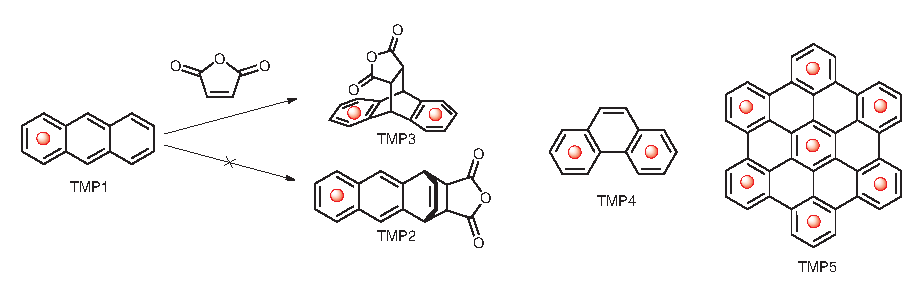
\includegraphics{figures/intro/clar.eps} 
				\caption[]{Examples of polycyclic aromatic hydrocarbons, and the application of Clar's rule to predict and rationalise aromatic character. The red dots denote aromatic sextets.}
				\label{fig:intro:clar}
			\end{figure}

			This idea has been extended to hexabenzocoronene (HBC)\nomenclature{HBC}{Hexabenzocoronene}, which has a maximum of seven aromatic sextets. Spectacularly, the different aromatic and single bond character predicted by Clar's rule is measurable by atomic force microscopy (AFM).\autocite{Gross2012}

			Porphyrins present another example of polycyclic aromaticity: they essentially comprise an [18]-annulene $[4n+2]$ \pii{}-electron pathway appended by two (spectator) ethylene bridges and two aromatic 6 \pii{}-electron pyrroles. Both of these aromatic ring current paths are important to the porphyrin aromaticity, though on an atom-weighted basis the pyrroles contribute more aromatic stabilisation energy.\autocite{Wu2013} %The relative stability conferred by the pyrrole aromaticity is sufficient to give a net aromatic stabilisation to a [20]-annulene (formally antiaromatic) with two fused pyrroles.\autocite{Wu2013}  
			The aromatic stabilisation energy (ASE) calculated by the block-localised wavefunction method to isolate the \pii{}-electron effects shows that the ASE from the macrocyclic [18] \pii{}-electron circuit in the porphyrin is the same as that of an individual 6 \pii{}-electron pyrrole (\SI{\sim 80}{\kilo\joule\per\mole}).\autocite{Wu2013}

		\subsubsection{Homoaromaticity}

			The homoaromatics comprise a different sort of topological perturbation of the monocyclic \pii{}-framework of the annulenes: introduction of an insulating (\ltt{e.g.} \ce{CH2}) interruption. Remarkably, aromaticity and conjugation can persist in charged species despite this disruption. So, the homotropylium cation \cmpd{homoarom} (\ce{C8H9+}, \autoref{fig:intro:aromatics}) is distinctly aromatic, as revealed by the different chemical shifts of protons 8 (inside, \SI{-0.6}{\ppm}) and 8\textprime{} (outside, \SI{5.2}{\ppm}).\autocite{Rosenberg1962,Gleiter2012}

			Homoaromaticity is much rarer for neutral species,\autocite{Gleiter2012} and seems to arise only when the \pii{}-orbitals on either side of the conjugation defect are close enough to effect delocalisation, such as in the theoretical trishomoaromatic molecule \cmpd{trishomoarom} (\autoref{fig:intro:aromatics}).\autocite{Stahl2002}

		\subsubsection{M\"obius aromaticity}

			Heilbronner (1964) predicted that the introduction of a \SI{180}{\degree} phase shift into the aromatic \pii{}-system would reverse H\"uckel's law: such a molecule with $[4n]$ \pii{}-electrons is then aromatic, and $[4n+2]$ \pii{}-electrons becomes antiaromatic.\autocite{Heilbronner1964} Such molecules are known as M\"obius aromatic molecules, for their resemblance to the topological M\"obius strip (\autoref{fig:intro:mobius}).

			\begin{figure}[ht!]
				\centering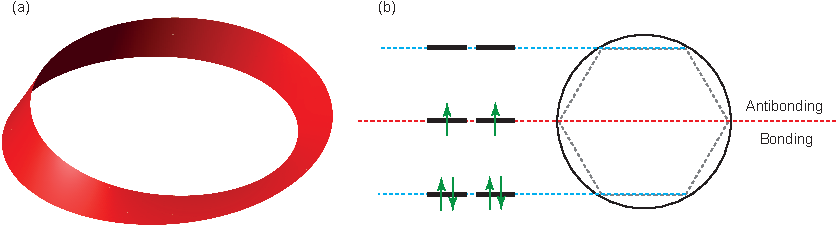
\includegraphics{figures/intro/mobius.pdf} 
				\caption[]{(a) A M\"obius strip. (b) A Frost-Musulin diagram for a hypothetical 6 \pii{}-electron M\"obius molecule.}
				\label{fig:intro:mobius}
			\end{figure}

			The first synthetic example of a M\"obius aromatic molecule was given by Herges and coworkers: the twisted [16]-annulene \cmpd{herges} (\autoref{fig:intro:mobiusstr}) is aromatic.\autocite{Ajami2003} It is possible to introduce two M\"obius twists into a molecule, at which point it reverts back to H\"uckel's aromaticity rules.\autocite{Fowler2006,Rzepa2005} Several examples of expanded porphyrins which exhibit M\"obius aromaticity have been reported by Osuka and co-workers.\autocite{Yoon2009a}



			\begin{figure}[ht!]
				\replacecmpd{herges}
				\centering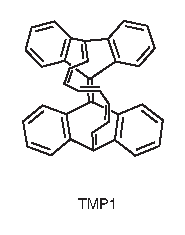
\includegraphics{figures/intro/mobius.eps} 
				\caption[]{Example of M\"obius aromatic compound \cmpd{herges}.\autocite{Ajami2003}}
				\label{fig:intro:mobiusstr}
			\end{figure}


		\subsubsection{Excited state aromaticity}

			In molecules which exhibit excited state (anti)aromaticity (ES(A)A), the electron-counting rules are once again reversed (\autoref{table:intro:arom}).\autocite{Baird1972,Rosenberg2014} The effect has been reported in expanded porphyrins by Osuka and co-workers, and was assigned on the basis of the structure of excited state absorption spectra.\autocite{Sung2015,Oh2016} In their case, an excited state aromatic compound has an absorption spectrum similar to a ground state aromatic analogue, and \ltt{vice versa} for excited state antiaromaticity. A further introduction to excited state aromaticity is given in \autoref{ch:excited-arom}.


			\begin{table}[!ht]
				\centering
				\caption[]{Effect of topology, \pii{}-electron count and electronic state on (anti)aromatic character.}
				\label{table:intro:arom}
				\begin{threeparttable}
					\begin{tabular}{lcccc}
						 & \multicolumn{2}{c}{Ground state} & \multicolumn{2}{c}{Excited state} \\
						 & $4n$ & $4n+2$ & $4n$ & $4n+2$ \\
						 \midrule
						 \textit{H\"uckel} & Antiaromatic & Aromatic & Aromatic & Antiaromatic \\ 
						 \textit{M\"obius} & Aromatic & Antiaromatic & Antiaromatic & Aromatic \\
						\bottomrule
					\end{tabular}
				\end{threeparttable}
			\end{table}


	\section{The limits of electron delocalisation}

		Aromaticity can be considered the limit of electron delocalisation in molecules: the ring-current model leads us to imagine that the \pii{}-electrons are freely circulating around the entire conjugation path. However, cyclic conjugation is not the sole requirement for aromaticity: the cycloparaphenylenes (CPP) and cycloparaphenyleneacetylenes (CPPA) do not exhibit measurable macrocyclic aromaticity around their peripheries,%
%
			\footnote{Taubert \ltt{et al.} have calculated the magnitude of macrocyclic ring currents in [6]-CPP to [11]-CPP and report paratropic and diatropic currents for [6]-CPP and [7]-CPP, respectively. These ring-currents do not significantly affect NICS(0) at the CPP ring centres (\SI{-2.1}{\ppm} and \SI{-1.9}{\ppm} for [6]- and [7]-CPP, respectively). The reversal of the calculated current direction between [6]- and [7]-CPP is surprising because both CPPs are, formally, $[4n]$ all-\textit{cis} annulenes. In contrast, the dianions  ($[4n+2]$ \pii{}-electrons) of all the CPPs studied are aromatic according to NICS(0).\autocite{Taubert2010}} %
		%
		as evidenced by their benzeniod NMR spectra.\autocite{Kawase2007,Jasti2011,Xia2012} Indeed, it is only upon oxidation to the dication that a ring current is observed in [8]-CPP.\autocite{Toriumi2015} Similarly to homoaromaticity in charged molecules, it seems that oxidation disrupts the ground state electronic character (8 isolated benzene rings) and permits enhanced delocalisation (a [32]-annulene dication with 30 \pii{}-electrons). 

		We are led to the inevitable question: if CPP does not exhibit macrocyclic aromaticity, how can porphine be aromatic? Porphine has three sources of aromatic stabilisation, all calculated to be of roughly equal weight (\SI{\sim 80}{\kilo\joule\per\mole} BLW-ASE (block-localised wavefunction)): the [18]-annulene pathway and two pyrroles.\autocite{Wu2013} The pyrrole aromaticity is not entirely `switched off' in favour of the [18]-annulene circuit, since there are still local pyrrolic ring currents. The same calculations predict a BLW-ASE for benzene of about \SI{120}{\kilo\joule\per\mole}, and for isolated pyrrole of about \SI{70}{\kilo\joule\per\mole}.\autocite{Wu2013} 

		There are two key differences between the CPP(A)s and porphine: first, there is much more ASE to be lost (about \SI{50}{\kilo\joule\per\mole}) by (partial) disruption of the local aromaticity of benzene than of pyrrole. Second, in the absence of an [18] \pii{}-electron circulation in porphine, the 12 non-pyrrolic \pii{}-electrons of the circuit are localised: essentially, there is a Pauling resonance argument for delocalising these additional electrons through macrocyclic aromaticity. In contrast, CPP has no localised electrons, and [$n$]-CPPA has a $6n$:$4n$ ratio of aromatic:static electrons. If a macrocyclic ring current were to be established in [$n$]-CPPA, only 4 \pii{}-electrons from each benzene would be involved, immediately negating the electron-counting benefit of including $2n$ acetylene electrons in the macrocyclic aromatic circuit.\autocite{Bleszynski-Jayich2009}

		As will be discussed in the introductions to Chapters \ref{ch:hexacat}, \ref{ch:excited-arom} and \ref{ch:truncnano}, large aromatic molecules are of interest because they may exhibit novel quantum effects, such as a Aharonov-Bohm oscillations of the ring current direction as a function of magnetic field.\autocite{Bleszynski-Jayich2009,Mayor2003} Such oscillations, introduced in more detail in \autoref{ch:hexacat}, could result in magnetic field control of conductance through a molecular junction.\autocite{Hod2006,Rai2011} Intriguingly, at high magnetic fields it has been calculated that molecular ring currents will reverse direction,\autocite{Soncini2004,Tellgren2009} just like the experimental observations in metal rings.\autocite{Chandrasekhar1991}

		Aromaticity and antiaromaticity are predominantly features of molecules with even numbers of electrons. For those with odd-numbers of electrons, such as radical cations and anions, the focus for studies of electron delocalisation is the radical electron/hole, or polaron. As we shall introduce more thoroughly in \autoref{ch:radcat}, the extent of charge (or spin) delocalisation is an important predictor of molecular properties in a device: with long delocalisation lengths, coherent transport becomes possible, preserving the quantum state of an injected electron or hole.\autocite{Heckmann2012} In contrast, shorter delocalisation lengths can still transmit charge over long distances along a molecular wire, through a stepwise hopping process.\autocite{Heckmann2012} Charge delocalisation has been reported to be `extreme' (across up to seven porphyrin units, \SI{7.5}{\nano\metre}) in monoalkyne-linked linear porphyrin oligomer radical cations and anions.\autocite{Susumu2006,Therien2015} Polyfluorenes (\textbf{PF}) have been extensively studied, and seem to have a radical anion delocalisation length of 3--5 fluorene units.\autocite{Takeda2006,Zaikowski2012,Bakalis2014} For poly(3-decylthiophene) (\textbf{P3DT}), the polaron delocalisation length is remarkably long: 11.5 units for an anion, or 8.7 units for a cation,\autocite{Takeda2012} though in terms of spatial extent (\SIrange{4}{5}{\nano\metre}) these distances are similar to those for \textbf{PF}. In contrast, the polaron delocalisation length is limited to 2--3 monomer units in a poly(phenylenevinylene) (\textbf{PPV}) radical anion.\autocite{Nguyen2010,Bakalis2014}

		\begin{figure}[ht!]
			\centering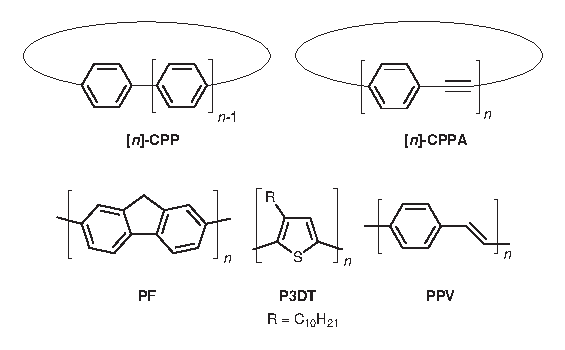
\includegraphics{figures/intro/polymers.eps} 
			\caption[]{Examples of conjugated polymers.}
			\label{fig:intro:polymers}
		\end{figure}

		Charge delocalisation is controlled by two competing effects: the conjugated \pii{}-system efficiently delocalises charge, but its efforts are frustrated by the presence of conjugation breaking defects. These defects can be kinks and twists in the oligomer chain,\autocite{Grozema2002} or can arise from a more dynamic vibrational relaxation following polaron formation: electron-phonon coupling. In this second case, a short segment of the oligomer chain becomes more strongly conjugated (lower BLA) and thus encourages charge localisation within this region.\autocite{Takeda2012} Overall, polaron delocalisation depends on \pii{}-conjugation, oligomer flexibility, and the absence of charge-localising vibrations.


%DFT on PPV. Effect of functional on delocalisation. In all cases singlet > polaron > triplet \autocite{Nayyar2011}

	\section{Prospective}

		The remainder of this thesis starts by considering perhaps the simplest case of delocalisation in butadiyne-linked porphyrin oligomers: the resonance energy of the neutral dimer \lp2 (\autoref{ch:dimer}). The resonance energy is determined from the experimentally determined height of the torsion barrier for rotation of porphyrins around the butadiyne link. \autoref{ch:dimer} also serves to introduce some of the photochemistry of porphyrins. 

		Next, we explore the chemistry of the even \pii{}-cations of the [6]-porphyrin nanoring \cp6 and its template complex \rwt6 (\autoref{ch:hexacat}). Although the nanoring does not exhibit global aromaticity (\ltt{i.e.} around the nanoring circumference) in its neutral oxidation state, after oxidation it is shown to obey H\"uckel's law. \cp6 exhibits aromaticity and antiaromaticity in its 6+ and 4+ oxidation states, respectively. It is even possible to generate the 12+ cation of the nanoring: this oxidation state corresponds to six antiaromatic ([16]-\pii{}) porphyrin subunits, and global (anti)aromaticity is not prominent. These conclusions are developed from DFT and experiment.

		We next turn to an exploration of charge and spin delocalisation in the radical cations of a series of linear (\lp1 to \lp6), cyclic (\cp6 and \rwt6) and tubular (\tubewt{}) porphyrin oligomers (\autoref{ch:radcat}). By using spectroelectrochemistry, DFT, and EPR, we show that the cation is delocalised over just two or three porphyrin units.

		The thesis concludes with two short chapters which each extend the study of aromaticity in porphyrin nanorings. In \autoref{ch:excited-arom} we ask whether porphyrin nanorings exhibit ES(A)A\@. Although DFT suggests that nanorings smaller than \cp8 do have ES(A)A, initial photophysical experiments do not reveal any physical manifestations. In the final chapter (\autoref{ch:truncnano}) we use DFT to calculate the effect of removing a single acetylene (\ce{C2}) unit from \cp6 -- does the nanoring still obey H\"uckel's rules when two \pii{}-electrons are removed, with an accompanying reduction in symmetry? The resulting molecule, with asymmetric conjugation paths, is interesting for studies on quantum interference. This chapter is entirely computational: synthetic efforts towards the truncated nanoring are under way independently. 



%Porphyrin with exocyclic double bonds in the meso positions is non-aromatic: just four aromatic pyrroles but no communication between them, just cross-conjugation.\autocite{Otto1991}

%Porphyrins with a pyridine in the macrocycle are non-aromatic \autocite{Abebayehu2016}

%!TEX root = ../thesis.tex
%!TEX spellcheck
\begin{savequote}[8cm]
I do not know what I may appear to the world, but to myself I seem to have been only like a boy playing on the sea-shore, and diverting myself in now and then finding a smoother pebble or a prettier shell than ordinary, whilst the great ocean of truth lay all undiscovered before me.
  \qauthor{--- Isaac Newton, as quoted in Memoirs of the Life, Writings, and Discoveries of Sir Isaac Newton (1855) by David Brewster (Volume II. Ch. 27)}
\end{savequote}


\chapter{\label{ch:dimer}Experimental and computational evaluation of the barrier to torsional rotation in a butadiyne-linked porphyrin dimer} 

\minitoc

\paragraph{Parts of this chapter were published in:} \fullcite{Peeks2016}. 

\enlargethispage{-2\baselineskip} \pagebreak

\section{Abstract}
	The barrier to torsional rotation in a butadiyne-linked porphyrin dimer in solution has been determined by variable temperature UV-Vis-NIR spectroscopy: $\delh = \SI{5.27 \pm 0.03}{\kjmol}$, $\dels = \SI{10.69 \pm 0.14}{\jkmol}$. The value of \delh agrees well with theoretical predictions. Quantum chemical calculations (DFT) were used to predict the torsion angle dependence of the absorption spectrum, and to calculate the vibronic fine structure of the \sing0$\rightarrow{}$\sing1 absorption for the planar dimer, showing that the absorption band of the planar conformer has a vibronic component overlapping with the $\langle0|0\rangle$ absorption of the perpendicular conformer. The torsion barrier in the porphyrin dimer is higher than that of 1,4-diphenylbutadiyne (calculated $\delh = \SI{1.1}{\kjmol}$). Crystallographic bond lengths and IR\nomenclature{IR}{Infra-red} vibrational frequencies confirm that there is a greater contribution of the cumulenic resonance form in butadiyne-linked porphyrin dimers than in 1,4-diphenylbutadiyne. The DFT frontier orbitals of the twisted conformer of the porphyrin dimer are helical, when calculated in the absence of symmetry. The helical character of these orbitals disappears when \symm{D}{2d} symmetry is enforced in the 90\textdegree{} twisted conformer. Helical representations of the frontier orbitals can be generated by linear combinations of the more localised orbitals from a symmetry-constrained calculation but they do not indicate $\pi$-conjugation. This work provides insights into the relationship between electronic structure and conformation in alkyne-linked conjugated oligomers. 

	%

\section{Introduction}
	Molecules with extended \pii-conjugation are of wide interest, both as ingredients in molecular electronic and optical materials,\autocite{Roncali1997,Pron2010} and as molecular wires for creating nanoscale electronic devices.\autocite{Tour2000,Carroll2002,Robertson2003,Metzger2015} Conjugated oligomers and polymers have been constructed by linking aromatic monomer units with a wide variety of \pii-conjugated bridges.\autocite{Martin1999} The properties of these oligomers are critically dependent on the molecular conformation because any twist in the \pii-system can dramatically reduce the coherent electronic coupling through the bridge. Conformational heterogeneity can thus attenuate the ability of a conjugated molecule to transport charge or electronic excitation. Several workers have explored the relationship between conformation and function in different types of molecular wire.\autocite{Martin1999,Davis2001,Yoshida2003,Venkataraman2006,Ahn2006,Chang2008,Kocherzhenko2012,Sun2014,Gilbert2015} Conjugated butadiyne-linked porphyrin oligomers have been actively investigated for more than twenty years,\autocite{Arnold1978,Arnold1992,Lin1994,Anderson1994,Lin1995} but the barrier to torsional rotation around the butadiyne link has yet to be determined experimentally. In this chapter, we present a time-dependent density functional theory (TD-DFT) evaluation of the electronic excitations of the porphyrin dimer as a function of inter-porphyrin torsion angle, and use variable temperature (VT) UV-Vis-NIR\nomenclature{UV}{Ultraviolet}\nomenclature{NIR}{Near IR} spectroscopy to determine the torsion barrier. Our experimental results permit the accurate simulation of conformational dynamics in this, and similar, systems. Our (TD-)DFT results provide insights into the nature of bonding and electronic excitations in butadiyne-linked oligomers.

	Porphyrin-based molecular wires have been widely investigated for their potential applications in functional materials,\autocite{Tanaka2015} as dyes for two-photon absorption,\autocite{Collins2008,Wilkinson2014} as models for biological photosystems (\ltt{e.g.} light-harvesting photosystem 2)\autocite{Nakamura2007} and as wires for single-molecule charge transport.\autocite{Sedghi2008,Sedghi2011,Sedghi2012} The Anderson group, and others, have prepared a wide variety of \textit{meso}--\textit{meso} butadiyne-linked porphyrin architectures, including linear oligomers,\autocite{Anderson1994,Lin1995,Taylor1998,Anderson1999} nanorings\autocite{Hoffmann2007,OSullivan2011} and supramolecular complexes.\autocite{Anderson1994,Taylor1999,Sprafke2011a} Other linking groups have also been explored: \textit{meso}--\textit{meso} alkynylene,\autocite{Lin1994} vinylene,\autocite{Frampton2005} phenylenes,\autocite{Lindsey1994,Wagner1995,Pawlicki2012} and direct porphyrin connection via oxidative coupling at the $\beta$ and \textit{meso} positions,\autocite{Tsuda2001} among many others. 

	The \textit{meso}--\textit{meso} butadiyne link permits strong inter-porphyrin electronic coupling and the extension of conjugation upon oligomer homologation is most apparent in the progressive bathochromic shift of the lowest energy optical transition (\sing0$\rightarrow{}$\sing1, 625–\SI{850}{\nano\metre}, Q-band, \autoref{fig:dimer:f1}). However, the butadiyne link also permits torsional heterogeneity, with a continuous range of torsion angles ($\theta$) between the porphyrin chromophores. The length of the butadiyne bridge is sufficient to avoid any steric repulsion between the opposing $\beta$ hydrogens of the porphyrins (denoted "X" in \autoref{table:dimer:t1}), thus the lowest energy conformer is planar ($\theta$ = 0\textdegree{}). The energy difference between the perpendicular and planar conformers reflects the bridge-mediated resonance stabilisation energy between the porphyrins. The torsional heterogeneity contributes towards the increasing width of the Q-band absorption with increasing oligomer length (\autoref{fig:dimer:f1}).

	\begin{figure}[ht!]
		\centering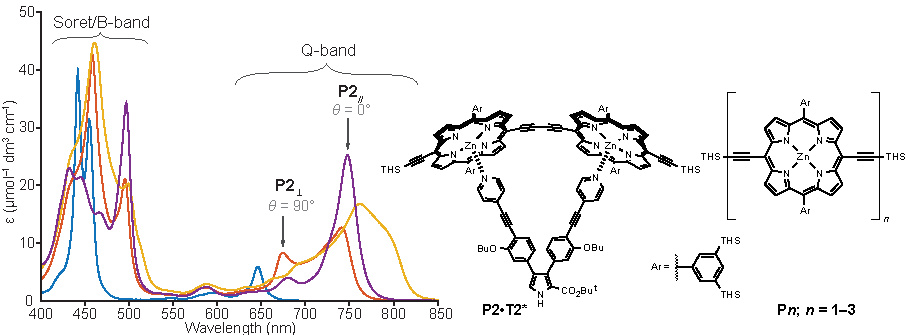
\includegraphics{figures/dimer/Figure-1.pdf} 
		\caption[]{Absorption spectra of linear oligomers: monomer \p1 (blue), dimer \p2 (red), trimer \p3 (yellow) and planar dimer complex \p2 $\bullet$ \textbf{T2} (purple). (Solvent: \ce{CH2Cl2}:THF:pyridine 10:10:1, except \p2$\bullet$\textbf{T2}: \dcm. THS = trihexylsilyl.)}
		\label{fig:dimer:f1}
	\end{figure}

	Previous semi-empirical and DFT calculations have predicted that the lowest energy conformation of \p2 is planar ($\theta = 0\degree$). These calculations gave a torsional energy barrier ($\Delta E$) of about \SIrange{3}{4}{\kjmol} (\autoref{table:dimer:t2}, \autoref{fig:dimer:f2}) between $\theta = 0\text{ and }90\degree$,\autocite{Lin1995,Stranger1996,Winters2007} which is in the range of $k_\text{B}T$ at room temperature (\SI{2.48}{\kjmol}), thus it is anticipated that all torsion angles are populated at room temperature. The barrier height was not significantly affected by the use of a range-separated DFT functional (CAM-B3LYP),\autocite{Yanai2004} an effective core potential, or a solvent model (\autoref{table:dimer:t2}). The torsion profile for the butadiyne linked dimer \p2 contrasts with that for the corresponding monoalkyne linked dimer\autocite{Lin1994}: in that case, coplanarity is disfavoured by the steric clash between porphyrin $\beta$ protons, and the DFT equilibrium torsion angle is about \SI{34}{\degree} (\autoref{fig:dimer:f2}). The $\Delta E$ between the equilibrium geometry and the perpendicular \SI{90}{\degree} conformer is around \SI{5}{\kilo\joule\per\mole}, greater than that in butadiyne linked \p2, and indicating increased conjugation across the linker. These computational results on \textbf{C\tsub2-}\p2 are in agreement with those found in several other studies, reviewed and contributed to by Rintoul \ltt{et al.},\autocite{Rintoul2013} who note that the computational equilibrium torsion angle (\textasciitilde{}\SI{35}{\degree}) is much greater than that expected from the narrow, redshifted absorption spectrum and than the angles observed in crystal structures (0--\SI{20}{\degree}).


	Computational work\autocite{Winters2007} (TD-DFT calculations, reproduced in this work, \autoref{fig:dimer:f4}) has shown that the visible electronic transitions of the butadiyne-linked porphyrin dimer exhibit a strong dependence on interporphyrin torsion angle $\theta$; as $\theta$ increases from 0 to 90\textdegree\ the Q-band transition is hypsochromically shifted. Torsion angle-dependence is also apparent in the B-band, albeit in the presence of several overlapping transitions.

	\begin{table}[ht!]
	\centering
		\caption[]{Molecular structures referred to in \autoref{table:dimer:t2} and in the present study}
		\label{table:dimer:t1}
	\begin{threeparttable}
	\begin{tabular}{ccccc}
	\multicolumn{5}{c}{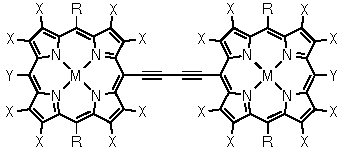
\includegraphics{figures/dimer/Table-1-Display.pdf}} \\
		\# & M & R & X & Y \\
		\midrule
		\cmpd{p2.a} & Ni & H & Et & H \\
		\cmpd{p2.b} & Zn & H & H & H \\
		\cmpd{p2.c} & Zn & Ph & H & \ce{C2H} \\
		\cmpd{p2.d} & Zn & Ph & H & \ce{C2SiMe3} \\
		\cmpd{p2.e}& Zn & H & H & \ce{C2H} \\
		\p2 & Zn & Ar\textsuperscript{\textdagger} & H & \ce{C2THS}\textsuperscript{\ddag} \\
		\bottomrule
	\end{tabular}
	\begin{tablenotes}
		\item \textdagger\ Ar $=$ 3,5-bis(trihexylsilyl) as defined in \autoref{fig:dimer:f1}. \item \ddag\ THS = trihexylsilyl.
	\end{tablenotes}
	\end{threeparttable}
	\end{table}

	\begin{table}[ht!]
	\centering
		\caption[]{Calculated barriers, $\Delta E$, to torsional rotation in butadiyne-linked porphyrin dimers}
		\label{table:dimer:t2}
	\begin{threeparttable}
	\begin{tabular}{cccc}
		Molecule & Method & $\Delta E$ (\si{\kjmol}) & Ref \\
		\midrule
		\cmpd{p2.a} & VWN and BP86 & $\sim\!63$ & \cite{Stranger1996} \\
		\cmpd{p2.b} & AM1 & $\sim\!4$ & \cite{Lin1995} \\
		\cmpd{p2.c} & B3LYP/6-31G* & 2.8 & \cite{Winters2007} \\
		\cmpd{p2.d} & B3LYP/6-31G*/LANL2DZ & 3.1\textsuperscript{\textdagger} & This work \\
		\cmpd{p2.d} & TPSSh/6-31G*/LANL2DZ & 3.7\textsuperscript{\textdagger}& This work \\
		\cmpd{p2.d} & CAM-B3LYP/6-31G* & 1.3\textsuperscript{\textdagger}& This work \\
		\cmpd{p2.d} & CAM-B3LYP/6-31G* \textsuperscript{\ddag} & 2.3\textsuperscript{\textdagger}& This work \\
		\cmpd{p2.d} & B3LYP/def2-SV(P) & 2.8\textsuperscript{\textdagger}& This work \\
		\cmpd{p2.e} & B3LYP/6-31G* & 2.6\textsuperscript{\textdagger}& This work \\
		\bottomrule
	\end{tabular}
	\begin{tablenotes}
		\item \textdagger\ No zero-point energy (ZPE)\nomenclature{ZPE}{Zero-point energy} correction applied. \item \ddag\ PCM\nomenclature{PCM}{Polarisable continuum model} THF solvent model.
	\end{tablenotes}
	\end{threeparttable}
	\end{table}



	\begin{figure}[ht!]
		\centering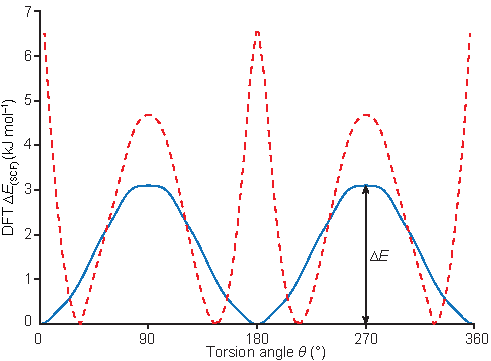
\includegraphics{figures/dimer/Figure-2b.pdf} 
		\caption[Calc. torsion profile for \p2]{Calculated (B3LYP/6-31G*/LANL2DZ) energy profile for butadiyne torsion in \p2, model \cmpd{p2.d} (blue). The red dashed line shows the torsion profile (B3LYP/6-31G*) for a monoalkyne linked analogue of \p2 (substitution pattern corresponding to model \cmpd{p2.b}). $\theta$ is the angle between the mean planes of each porphyrin, defined by the 24 non-hydrogen atoms in each macrocycle. The indicated $\Delta E$ is the torsional barrier for \p2 which is under discussion in this chapter.}
		\label{fig:dimer:f2}
	\end{figure}

	The torsion-dependence of the Q-band absorption wavelength has been exploited to selectively excite populations of molecules with different conformations. The wavelength of fluorescence emission is also dependent on the torsion angle. Analysis of fluorescence emission and excitation spectra shows that the \sing{1} state has a much higher torsion barrier (\SI{16}{\kjmol}) than the electronic ground state (\sing0).\autocite{Winters2007} Perpendicular conformers which are excited to \sing{1} tend to planarise prior to emission, unless solvent viscosity retards the rotation.\autocite{Winters2007,Kuimova2009,Kuimova2009b,Vyvsniauskas2015} The torsion angle has also been found to influence the two-photon absorption (2PA)\nomenclature{2PA}{Two-photon absorption} cross-section and the singlet oxygen (\ce{^{1}O_2}) yield. Planar conformers have stronger two-photon absorption,\autocite{Wilkinson2014} larger third-order optical non-linearities\autocite{Drobizhev2006} and higher charge-mobilities,\autocite{Grozema2007,Winters2007b} and they are more efficient oxygen sensitizers because intersystem crossing (\sing{1}$\rightarrow{}$\trip{1}) is faster than in twisted conformers.\autocite{Kuimova2009}

	The torsion angle can be constrained to enforce coplanarity by the preparation of supramolecular complexes, such as ladder complexes with a bidentate ligand (\ltt{e.g.} DABCO or 4,4\textprime-bipyridine),\autocite{Taylor1999} or simple 1:1 complexes between oligomers and designed templates, such as \textbf{T2} (\autoref{fig:dimer:f1}).\autocite{Winters2007,Winters2007b} Fixing the torsion angle results in the expected bathochromic shift and sharpening of the Q-band (\autoref{fig:dimer:f1}), as the conformation is restricted to a librational range of angles around $\theta \approx 0\degree$.

	Interestingly, Aida \ltt{et al.}\ prepared tetrameric cages from \textit{meso}-pyridyl substituted butadiyne-linked porphyrin dimers.\autocite{Tsuda2005} They found that the cage composed of dimer units with perpendicular porphyrins was favoured, due to the resulting cancellation of the pyridine dipole moments. This result showed that the torsion barrier in the butadiyne-linked dimer is low enough to be overcome by a dipole-based conformational preference.\autocite{Tsuda2005}

	The aim of this chapter is to experimentally determine the barrier to torsion in porphyrin dimer \p2 using VT UV-Vis-NIR spectroscopy and to understand how torsional rotation alters the electronic structure of this molecule. After presenting the VT UV-Vis-NIR results, we will discuss our theoretical analysis of the electronic excitations. With the help of this theoretical analysis, we will extract thermodynamic parameters using a van't Hoff analysis. We will use evidence from IR spectroscopy and bond-length alternation to discuss the resonance stabilisation of the planar conformer. Finally, we discuss our observation of helical frontier orbitals and natural transition orbitals in DFT calculations. 
	\FloatBarrier

	\section{Methods}

	\subsection{Synthesis and spectroscopy}

		Porphyrin compounds were prepared as described previously.\autocite{Grozema2007,Tait2015} Oligomers \textbf{P\textit{N}} with trihexylsilyl (THS) solubilising groups on the \textit{meso}-aryls were used throughout this study, since THS porphyrins exhibit excellent solubility and a low propensity towards aggregation. Room temperature UV-Vis-NIR spectra were recorded using a Perkin-Elmer Lambda 20 with a \SI{1}{\centi\metre} quartz cuvette. Variable temperature UV-Vis-NIR spectra were recorded using a Perkin-Elmer Lambda 1050 and an Oxford Instruments L\ce{N2} optical cryostat, with \SI{1}{\centi\metre} and \SI{1}{\milli\metre} Infrasil Quartz cuvettes (Starna). In all cases, freshly mixed \ce{CH2Cl2}:THF:pyridine (10:10:1) was used as the solvent mixture. \dcm and THF\nomenclature{THF}{Tetrahydrofuran} were dried over activated alumina before use. \dcm contained amylene (\SIrange{50}{150}{\ppm}) as a stabiliser; THF was unstabilised. Variable temperature UV-Vis-NIR experiments were performed across a wide concentration range (\SI{0.8}{\micro\Molar}, \SI{1.6}{\micro\Molar} and \SI{58.5}{\micro\Molar}) to confirm the absence of thermally-induced aggregation. Absorbances were not corrected for concentration change due to thermal contraction of the solvent, since the ratio of absorbances is not affected by concentration. Emission spectra were collected using an ISA Fluoromax-2 Fluorimeter. Infrared spectra were collected using a Bruker Tensor 27 FT-IR\nomenclature{FT}{Fourier transform} spectrometer in ATR mode with neat sample, with \SI{2}{\wn} resolution at \SI{293}{\kelvin}.

		%

	\subsection{Computational methods}

		All (TD-)DFT calculations were conducted using Gaussian09/D.01.\autocite{g09} The B3LYP density functional\autocite{Becke1993} was used in conjunction with the 6-31G* basis set,\autocite{Ditchfield1971,Hehre1972,Hariharan1973,Rassolov1998} with the LANL2DZ ECP\autocite{Hay1985a,Hay1985}\nomenclature{ECP}{Effective core potential} on Zn as indicated. For computational tractability, truncated model compounds were used. The potential-energy surface scan and TD-DFT calculations used a model of \p2 with phenyl substituents in place of the \textit{meso}-aryls, and trimethylsilyl protecting groups as the acetylene end-groups, and \symm{C}{1} symmetry, \cmpd{p2.d}. Further truncated models were used for the calculation of the vibronic fine structure of the Q-band transitions and vibrational frequencies: the \textit{meso}-aryls and the trimethylsilyl acetylene protecting groups were replaced by hydrogens, \cmpd{p2.e}. These calculations were then conducted in \symm{D}{2h} and \symm{D}{2d} symmetry for planar and perpendicular conformers respectively.

		The potential energy surface was calculated by varying the interporphyrin torsion angle in 2.5\textdegree{} increments and, while holding the torsion coordinate fixed, relaxing the remainder of the structure. The resulting $\Delta E_{SCF}$ is used for comparison: the zero-point vibrational contribution to the energy has been neglected unless indicated otherwise. Vibrational frequencies (calculated analytically, with the harmonic oscillator model) were scaled by a multiplicative factor of 0.96.

		Unless otherwise specified, orbital isosurfaces are depicted using the default threshold settings in the Chimera\autocite{pettersen2004ucsf} program. Namely, the thresholds are placed symmetrically about zero, at a value which encompasses 99\% of the voxels on either side of zero. 


\section{Results and discussion}
	\subsection{Experimental VT UV-Vis-NIR spectroscopy}

		Since the calculated torsion barrier $\Delta E$ is of the order of $k_{\text{B}} T$ at room temperature, we envisioned that VT UV-Vis-NIR spectroscopy would probe the equilibrium between twisted and planar conformers. Indeed, dramatic changes in the UV-Vis-NIR spectrum of \p2 (\SI{\sim{}59}{\micro\Molar}, \ce{CH2Cl2}:THF:pyridine 10:10:1) were observed upon cooling within the solvent liquid range (298–\SI{173}{\kelvin}, \autoref{fig:dimer:f3}). Below \SI{180}{\kelvin}, discontinuous changes in the spectra are observed, which we attribute to changes in bulk solvent properties at temperatures close to the glass transition temperature.\autocite{Bublitz1998}

		\begin{figure}[ht!]
			\centering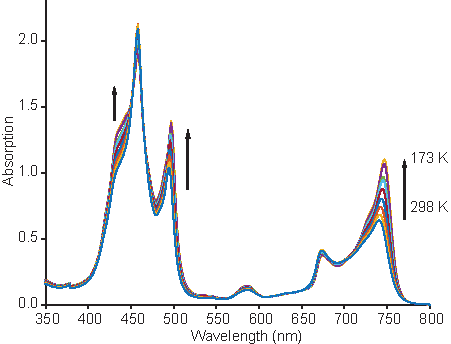
\includegraphics{figures/dimer/Figure-3.pdf} 
			\caption[]{Variable temperature (298–\SI{173}{\kelvin}) absorption spectra of porphyrin dimer \p2 in \ce{CH2Cl2}:THF:pyridine (10:10:1), concentration \ltt{ca.} \SI{59}{\micro\Molar}, path length \SI{1}{\milli\metre}.}
			\label{fig:dimer:f3}
		\end{figure}

		Previous work has shown that temperature-dependent changes in the absorption spectra of butadiyne-linked porphyrin oligomers can be caused by aggregation,\autocite{Karnbratt2012,Hutin2013} but as noted in the Methods, we were able to exclude the presence of aggregation by selection of appropriate solvent and solubilising side-chains. VT experiments performed on the porphyrin monomer \p1 in the same solvent mixture showed that, within the temperature range \SIrange{298}{163}{\kelvin}, there is no thermochromic shift of the Q-band absorption $\lambda$\textsubscript{max} (\autoref{fig:dimer:s1}).

		\begin{figure}[ht!]
			\centering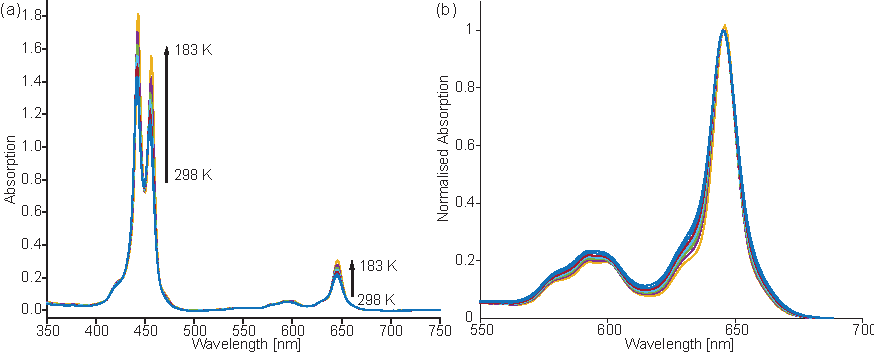
\includegraphics{figures/dimer/si-p1-vt-f1.pdf} 
			\caption[]{VT UV-­Vis spectra of monomer \p1 in \ce{CH2Cl2}:THF:pyridine 10:10:1, (a) full spectrum in temperature range
				298–77 K (b) expansion of Q-­band region in temperature range 298–\SI{163}{\kelvin}.}
			\label{fig:dimer:s1}
		\end{figure}

		When a solution of \p2 is cooled, its UV-Vis-NIR spectrum exhibits several changes (\autoref{fig:dimer:f3}): the red edge of the Q-band becomes more intense (\textasciitilde{}\SI{740}{\nano\metre}; planar conformations, $\theta \approx 0\degree$), at the expense of a slight decrease in intensity on the blue edge (\SI{675}{\nano\metre}; perpendicular conformations, $\theta \approx 90\degree$). We can be confident in our assignment of the absorbance at \SI{675}{\nano\metre} to perpendicular conformers thanks to measurements of the emission of twisted dimer conformers in viscous solution by Kuimova \ltt{et al.}\autocite{Kuimova2009b}, who found that highly viscous solvents inhibited excited state planarisation. The resulting emission, predominantly from twisted conformers, occurred bathochromically to the “shoulder” on the high-energy side of the Q-band absorption. 

		The absorption at \SI{570}{\nano\metre}, assigned with the help of TD-DFT to near-planar conformers (see later), increases intensity on cooling. In the Soret/B-band, a sharpening and intensification of the absorption on the red edge is observed (\textasciitilde{}\SI{490}{\nano\metre}). This band can thus also be assigned to near-planar conformers. Before discussing the van't Hoff analysis of the VT UV-Vis-NIR of \p2, we will further develop our understanding of the absorption spectra using TD-DFT\@.
		\FloatBarrier
	\subsection{Calculated electronic transitions as a function of torsion angle}

		We computed the electronic excitations for different torsion angles using TD-DFT (B3LYP/6-31G*/LANL2DZ) (\autoref{fig:dimer:f4}). The results agree with earlier published work.\autocite{Winters2007} The transition dipole moments for the lowest energy part of the Q-band are polarised along the butadiyne (long, \textit{x}) axis, as observed experimentally.\autocite{Anderson1994a,Drobizhev2005} Analysis of the angle dependence of the Q-band excitation energy reveals a relationship to $\cos \theta$: \ltt{i.e.}, the projection of the porphyrin planes (\autoref{fig:dimer:f5}), as given by equation (\ref{eqn:qband-cos}):

		\begin{figure}[ht!]
			\centering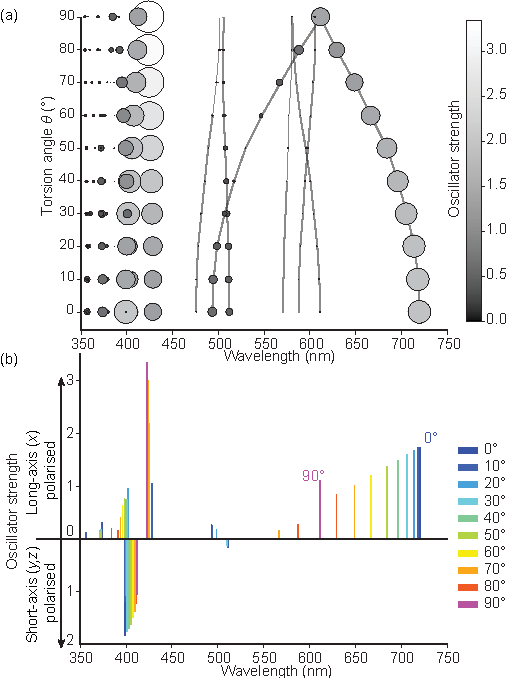
\includegraphics{figures/dimer/Figure-4.pdf} 
			\caption[]{Calculated (TD-B3LYP/6-31G*/LANL2DZ) vertical excitation energies in the UV-Vis-NIR region for different torsion angles in a model \p2 (\cmpd{p2.d}). (a) Calculated wavelength \ltt{vs.} torsion angle. Faint grey lines (only shown for the Q-bands) connect corresponding states, comprising a Walsh diagram; circle size is proportional to oscillator strength, as is the circle shading. (b) Calculated wavelength \ltt{vs.} oscillator strength. Transitions with oscillator strength \textless 0.1 are not included. Bars above the x-axis correspond to transitions polarised along the long molecular axis ($x$, butadiyne axis) of the molecules. Bars below the $x$-axis correspond to transitions polarised along either the $y$ or $z$ (short) molecular axes.}
			\label{fig:dimer:f4}
		\end{figure}

		\begin{figure}[ht!]
			\centering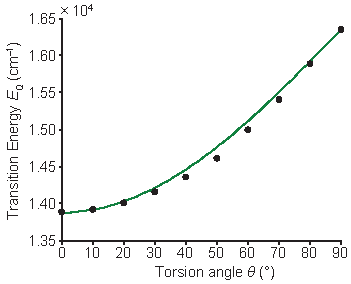
\includegraphics{figures/dimer/Figure-5.pdf} 
			\caption[]{Comparison of TD-DFT calculated \sing0$\rightarrow{}$\sing1 vertical excitation energy (blue) \ltt{vs.} a predictive model based on the projection of the porphyrin planes (green) (\eref{eqn:qband-cos}).}
			\label{fig:dimer:f5}
		\end{figure}

		\begin{equation}\label{eqn:qband-cos}
		E_Q \approx E_\bot - (E_\bot - E_\parallel)\cdot \cos \theta
		\end{equation}

		\noindent{}where $E_Q$ is the Q-band absorption energy for a conformer with inter-porphyrin torsion angle $\theta$. $E_\parallel$ and $E_\bot$ are the limiting energies for planar (low energy) and perpendicular (high energy) conformers, respectively. This function readily relates absorption energy to the overlap of the porphyrin \pii-systems along the butadiyne and shows that $E_Q$ is most sensitive to $\theta$ when $\theta \approx 90\degree$.

		The calculated oscillator strength of the lowest energy transition is surprisingly high for the 90\textdegree{} conformer (\autoref{fig:dimer:f4}b), contrasting its gradual decrease with increasing $\theta$ between 0–80\textdegree{}. This result does not appear to be a simple computational artefact: the increase of oscillator strength is gradual from 85--90\textdegree{} (\autoref{fig:dimer:s2}). Close examination of the TD-DFT results reveals that, on twisting from 0--90\textdegree{}, the second-lowest energy \textit{x}-axis (long axis) polarised transition is progressively redshifted until it becomes degenerate with the lowest energy transition (\autoref{fig:dimer:f4}a). This analysis further reveals that the weak absorption centred at \textasciitilde{}\SI{580}{\nano\metre} in the experimental spectrum (\autoref{fig:dimer:f1}) arises predominantly from planar conformers, and contains components polarised along both the long (\textit{x}) and short (\textit{y}) molecular axes. A detailed discussion of TD-DFT results and orbital/state correlations as a function of torsion angle has been published previously by Winters \ltt{et al.}, and our computational results are in complete agreement with theirs.\autocite{Winters2007}

		\begin{figure}[ht!]
			\centering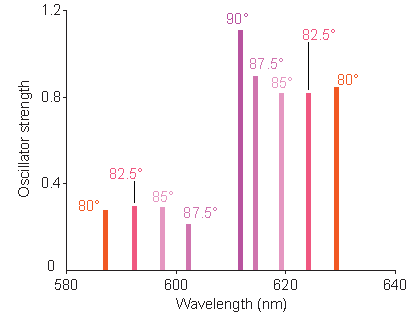
\includegraphics{figures/dimer/si-small-angles-f2.pdf} 
			\caption[]{TD-DFT (B3LYP/6-31G*/LANL2DZ) calculated excitation energies and oscillator strengths for \p2 (model \cmpd{p2.d}) as a function of inter-­porphyrin torsion angle}
			\label{fig:dimer:s2}
		\end{figure}

		The high oscillator strength of the Q band of the perpendicular conformer ($\theta = 90\degree$) provides a partial explanation for the peak observed in the absorption spectrum at \SI{675}{\nano\metre} (\figplural \ref{fig:dimer:f1} and \ref{fig:dimer:f3}). However, a further contribution appears likely because the peak at \SI{675}{\nano\metre} persists at low temperature, with similar relative intensity to the planar conformer as at room temperature. Even at \SI{78}{\kelvin}, at which temperature occupation of the perpendicular state should be thermally inhibited, there is a discrete absorption at \textasciitilde{}\SI{675}{\nano\metre} (\autoref{fig:dimer:f6}). Room temperature emission spectra of \p2 and \p2$\bullet$\textbf{T2} (\figplural \ref{fig:dimer:s7comb}a and \ref{fig:dimer:s7comb}b) show a similar shoulder on the red edge of the main emission band. Therefore we assign this shoulder to a vibronic contribution of the planar conformer, with the support of computational results described in the next section.

		\begin{figure}[ht!]
			\centering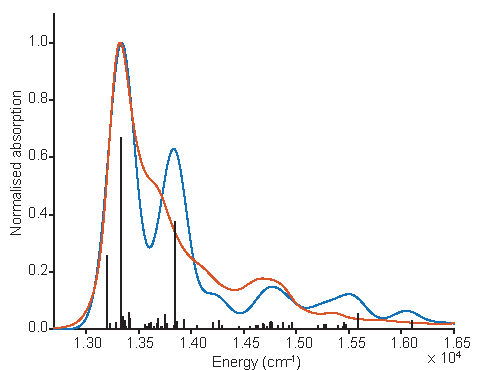
\includegraphics{figures/dimer/Figure-6.pdf} 
			\caption[]{(red) Absorption spectrum of Q-band region (600–\SI{800}{\nano\metre}) of \p2 in frozen solution (\ce{CH2Cl2}:THF:pyridine 10:10:1) at \SI{78}{\kelvin}; (blue) calculated (B3LYP/6‑31G* Franck-Condon/Herzberg-Teller approximation) vibronic structure of Q-band absorption for planar \p2, model \cmpd{p2.e}; (sticks) vibronic transitions; transitions with low relative intensity are not plotted. The $\langle0|0\rangle$ transition in the computational result was shifted in energy to match the low-energy peak in the experimental spectrum (red).}
			\label{fig:dimer:f6}
		\end{figure}

		\begin{figure}[ht!]
			\centering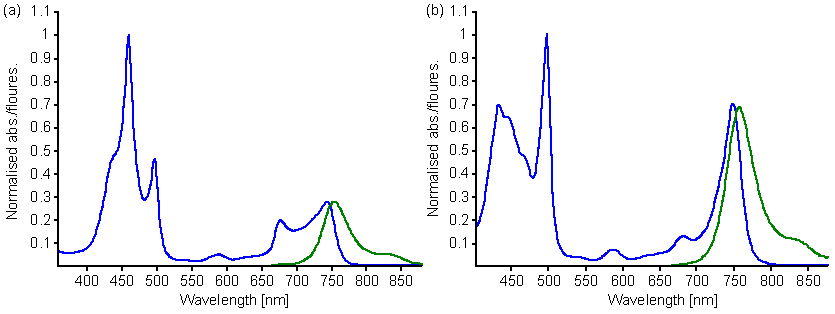
\includegraphics{figures/dimer/si-p2fl-comb.pdf} 
			\caption[]{Absorption (blue) and fluorescence (green) of (a) \p2 (\ce{CHCl3} + 1\% pyridine), $\lambda_{ex} = 450$ nm and (b) \p2$\bullet$\textbf{T2} (\ce{CHCl3}), $\lambda_{ex} = 450$ nm, $\lambda_{max}(\log_{10} \epsilon)$: 749 (5.297), 682 (4.574), 588 (4.324), 498 (5.452), 434 (5.295).}
			\label{fig:dimer:s7comb}
		\end{figure}

		\FloatBarrier
	\subsection{Vibronic contribution to the Q-band electronic transition}

		We used the Franck-Condon (FC)\nomenclature{FC}{Franck-Condon} and Herzberg-Teller (HT)\nomenclature{HT}{Herzberg-Teller} approximations as implemented in Gaussian09/D.01 to calculate the vibronic absorption spectrum for the \sing0$\rightarrow{}$\sing1 transition in planar \p2.\autocite{Santoro2008,Barone2009} The calculation was restricted to excitations originating from the vibrational ground state of \sing0, thus treating the vibronic spectrum as temperature independent. This calculation gave a predicted spectrum which is in remarkably close agreement to the experimental spectrum of \p2 recorded at \SI{78}{\kelvin} (\autoref{fig:dimer:f6}). At this temperature the near-planar conformers of \p2 are expected to be dominantly populated. The major vibronic bands arise from intra-porphyrin collective stretching modes, and do not appear to involve nuclear displacements on the butadiyne link (see \autoref{fig:dimer:s3}). The vibronic band which we calculate at \SI{\sim 390}{\wn} from the $\langle0|0\rangle$ transition has also been experimentally characterised by Camargo \ltt{et al.}\ in \p1, at \SI{380}{\wn}.\autocite{Camargo2015} We used the computational vibronic spectrum to firmly assign the absorption at \SI{675}{\nano\metre} in (planar) \p2$\bullet$\textbf{T2} (\autoref{fig:dimer:f1}) to a vibronic contribution. Similarly, the anomalously increased intensity at the blue edge of the Q-band (\textasciitilde{}\SI{675}{\nano\metre}) in the experimental spectra of \p2 at room temperature (\autoref{fig:dimer:f1}) is partially attributed to this vibronic contribution, in addition to the relatively high oscillator strength of the overlapping perpendicular absorption. The significant overlap between the absorption of the twisted conformer and that of a vibronic band of the planar conformer rationalises previous results where wavelength-selective excitation of the twisted conformer appeared to result, additionally, in excitation of the planar conformer.\autocite{Winters2007,Wilkinson2014} 

		\begin{figure}[ht!]
			\centering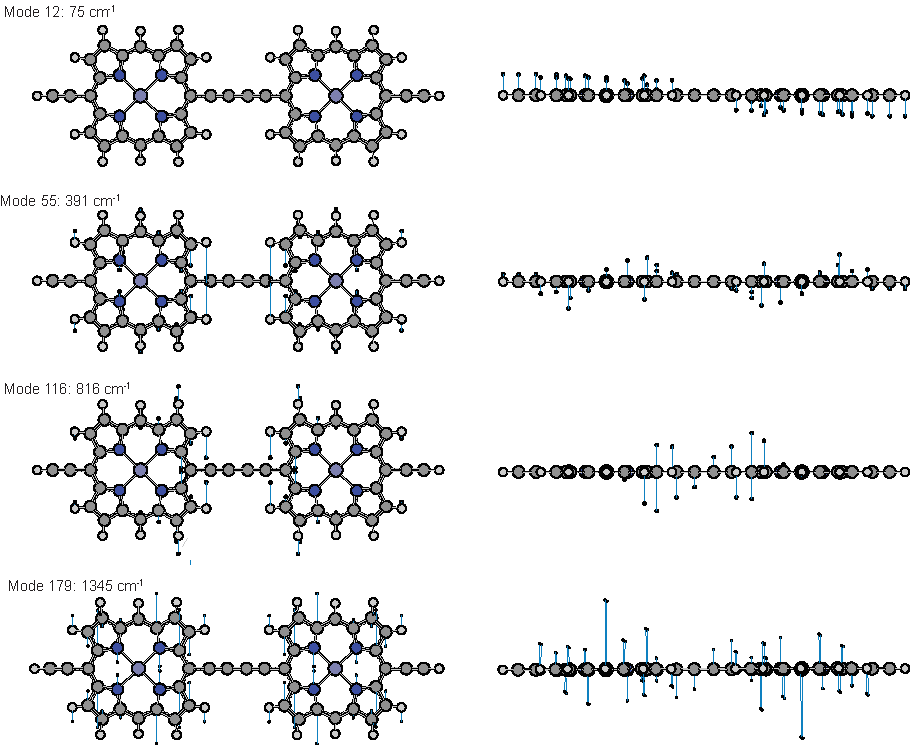
\includegraphics{figures/dimer/si-vibrations-s3.pdf} 
			\caption[]{Normal modes of \sing1 state of \p2 (model \cmpd{p2.e}) associated with major vibronic bands.}
			\label{fig:dimer:s3}
		\end{figure}
		\FloatBarrier
	\subsection{van't Hoff analysis of experimental VT UV-Vis-NIR data}

		The experimental VT UV-Vis-NIR data were subject to a van't Hoff analysis of the equilibrium constant for a simple two-state model comprising near-planar and near-perpendicular conformers, \p2$_\parallel$ ($\theta \approx 0\degree$) and \p2$_\bot$ ($\theta \approx 90\degree$) with concentrations proportional to the absorbances at 750 and \SI{675}{\nano\metre}, respectively, weighted by the TD-DFT oscillator strengths for the 0\textdegree{} and 90\textdegree{} transitions.\footnote[3]{We also used the van't Hoff equation without weighting the absorbances at 750 and \SI{675}{\nano\metre} to the calculated oscillator strengths.  This approach does not change the resulting value of \delh{} ($\SI{5.27 \pm 0.03}{\kjmol}$), but it gives a higher value of \dels{} ($\SI{14.42 \pm 0.14}{\jkmol}$); thus, $\Delta{}G_{\text{298 K}}$ becomes $\SI{0.98 \pm 0.05}{\kjmol}$ } The vibronic contribution of the planar conformer to the absorption at \SI{675}{\nano\metre} (mostly perpendicular conformer) was subtracted. The relative magnitude of this vibronic contribution was assumed to be temperature-invariant and was calculated from the ratio of peak heights in the spectrum of \p2 at \SI{78}{\kelvin}. 

		The equilibrium constant at each temperature was thus calculated according to equation (\ref{eqn:eqconstant}):

		\begin{equation}\label{eqn:eqconstant}
		K = \frac{f_\parallel}{f_\bot} \cdot \frac{A_\bot}{A_\parallel} = \frac{f_\parallel}{f_\bot} \cdot \frac{A_{675} - A_{750} \cdot x_{vibr}}{A_{750}}
		\end{equation}

		where $K$ is the equilibrium constant for:
		\begin{center}
			\ce{\textbf{P2}_$\parallel$ <=>[{$K$}][] \textbf{P2}_$\bot$}
		\end{center}

		$A_\parallel$ and $A_\bot$ are the absorbances for planar and perpendicular conformers, respectively. $f_\parallel$ and $f_\bot$ are the TD-DFT oscillator strengths for planar and perpendicular conformers, respectively ($\frac{f_\parallel}{f_\bot} = 1.574$). $x_{vibr}$ is the ratio of the intensities of the planar $\langle0|0\rangle$ absorption and its vibronic contribution (at \SI{\sim 1350}{\wn} separation) in the experimental \SI{78}{\kelvin} spectrum of \p2 ($x_{vibr} = 0.186$). The ratio of TD-DFT oscillator strengths (1.574) is consistent with the ratio of estimated experimental extinction coefficients for the planar and perpendicular conformers. The experimental ratio of extinction coefficients for planar and perpendicular conformers ($\frac{\epsilon_{\parallel}}{\epsilon_{\bot}}$) was estimated by comparing the absorption coefficients of free \p2 (in the presence of pyridine) and complexed \p2$\bullet$\textbf{T2} at \SI{750}{\nano\metre} (planar, $\epsilon_{\parallel}$) and \SI{675}{\nano\metre} (perpendicular, $\epsilon_{\bot}$), after subtraction of the vibronic contribution at \SI{675}{\nano\metre} in free \p2. The vibronic contribution in liquid solution at room temperature is given by the following equation, assuming that in \p2$\bullet$\textbf{T2}, there is no perpendicular \p2 (\ltt{i.e.}, all absorption at \SI{675}{\nano\metre} arises from the vibronic contribution).

		\begin{equation}
			x_{vibr}= \frac{\epsilon_{\SI{675}{\nano\metre}, \textbf{T2}}}{\epsilon_{\SI{750}{\nano\metre}, \textbf{T2}}} = 0.171
		\end{equation}

		Thus $\epsilon_\bot$ can be estimated by subtracting this vibronic contribution:

		\begin{equation}
			\epsilon_{\bot, py} = x_{vibr} \times \epsilon_{\SI{675}{\nano\metre}, py} = \SI{60960}{\per\Molar\per\centi\metre} 
		\end{equation}

		Where $\epsilon_{py}$ corresponds to spectra recorded in the presence of pyridine, and $\epsilon_{\textbf{T2}}$ to the complex \p2$\bullet$\textbf{T2}. Next we calculate $\Delta \epsilon_\parallel$. $\Delta \epsilon_\bot$ was found in the previous step (\SI{60960}{\per\Molar\per\centi\metre}) assuming all \p2 has been planarised.

		\begin{equation}
			\Delta \epsilon_\parallel = \epsilon_{\SI{750}{\nano\metre}, \textbf{T2}} = \epsilon_{\SI{750}{\nano\metre}, py} = \SI{103990}{\per\Molar\per\centi\metre} 
		\end{equation}

		Thus:

		\begin{equation}
		\frac{\Delta \epsilon_\parallel}{\Delta \epsilon_\bot} = \frac{\num{103990}}{\num{60960}} = 1.7059
		\end{equation}


		Within the temperature range 298–\SI{198}{\kelvin}, the van't Hoff plot (\autoref{fig:dimer:f7}) of the extracted equilibrium constants shows an excellent straight-line fit, and is concentration independent across the range measured (\SIrange{0.8}{59}{\micro\Molar}), thus excluding the presence of aggregation. Thermodynamic parameters were extracted: $\delh = \SI{5.27 \pm 0.03}{\kilo\joule\per\mole}$ (in reasonable agreement with most computational estimates, \autoref{table:dimer:t2}), $\dels = \SI{10.69 \pm 0.14}{\joule\per\kelvin\per\mole}$. The large value of \dels demonstrates an important temperature dependence for the rotational barrier: $\Delta G_{\SI{298}{\kelvin}} = \SI{2.08 \pm 0.05}{\kilo\joule\per\mole}$;  $\Delta G_{\SI{180}{\kelvin}} = \SI{3.35 \pm 0.04}{\kilo\joule\per\mole}$ -- in other words, the barrier rises as the temperature falls.

		\begin{figure}[ht!]
			\centering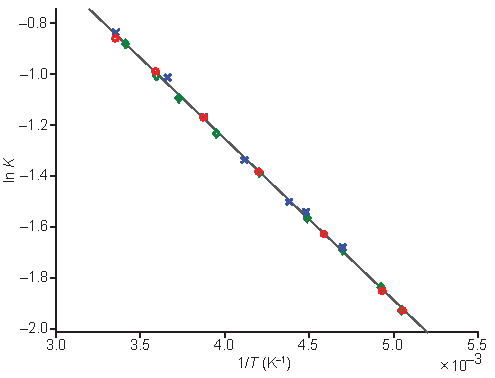
\includegraphics{figures/dimer/Figure-7.pdf} 
			\caption[]{van't Hoff plot and fit line for VT experiments at three different concentrations: \SI{0.8}{\micro\Molar} (blue crosses), \SI{1.6}{\micro\Molar} (green diamonds), \SI{58.5}{\micro\Molar} (red circles). $R^{2} = 0.999$.}
			\label{fig:dimer:f7}
		\end{figure}

		There are few previous reports of the determination of both \delh and \dels for a torsional equilibrium. Our thermodynamic parameters for \p2 are similar to those reported for \textit{trans}-\textit{skew} isomerism in 1,1-dihalo-3-fluoro-buta-1,3-dienes from solution-phase IR spectroscopy (halo = Br: $\delh = \SI{3.53}{\kilo\joule\per\mole}$, $\dels = \SI{3.5}{\joule\per\kelvin\per\mole}$; halo = Cl: $\delh = \SI{2.95}{\kilo\joule\per\mole}$, $\dels = \SI{2.3}{\joule\per\kelvin\per\mole}$).\autocite{Hartman1968} \dels for oxalyl chloride (\textit{trans}-\textit{gauche} isomerism) has been calculated from the experimental vibrational modes (excluding the torsion mode) as \SI{\sim{}13}{\jkmol},\autocite{Durig1992} and from gas-phase electron diffraction as \SI{10}{\jkmol}.\autocite{Hagen1973} We attribute our positive value of \dels to changes in the frequencies of large-amplitude (low frequency) motions between the planar and twisted states, including the pertinent torsion mode and butadiyne bending modes.

		The potential energy surface from DFT calculations (\autoref{fig:dimer:f2}) was scaled based on the experimentally determined thermodynamic parameters (\delh and \dels), and the Boltzmann equation (\autoref{eqn:dimer:boltz}) was used to determine the temperature dependence of the mole fraction of each conformer (\autoref{fig:dimer:f8}). Inclusion of the entropic factor in this manner permits a more accurate simulation of temperature-dependent populations than simply using a temperature-independent barrier height, which would overestimate conformational heterogeneity at low temperature, and underestimate it at high temperatures.

		\begin{equation}\label{eqn:dimer:boltz}
			%\frac{N_j}{N_i} = \frac{g_j}{g_i} \me^{-\frac{E_j - E_i}{k_\text{B}T}}
			p_i = \frac{\me^{-\frac{E_i}{k_\text{B}T}}}{\sum_{j=1}^M \me^{-\frac{E_j}{k_\text{B}T}}}
		\end{equation}
		\noindent{}where $p_i$ is the population of the $i$\nth state, $k_\text{B}T$ is the Boltzmann constant, and $E_i$ is the relative energy of the $i$\nth state. 

		\begin{figure}[ht!]
			\centering\includegraphics{figures/dimer/Figure-8.pdf} 
			\caption[]{Temperature dependence of the population density for different torsion angles, based on the experimentally determined \delh and \dels.}
			\label{fig:dimer:f8}
		\end{figure}

		The stated error in our thermodynamic parameters is the error in the fit of the experimental data to the van't Hoff equation, and must be taken in the context of the approximation of the two-state model. Our analysis presents a lower bound for the torsion barrier height, because the model evaluates the barrier between near-planar and near-perpendicular conformers. Spectral overlap between angles in a small range (estimated 0–20\textdegree{}) around 0\textdegree{} and 90\textdegree{} means that the absorptions at \SI{750}{\nano\metre} and \SI{675}{\nano\metre} capture some contributions from nearby angles.
		\FloatBarrier
	\subsection{Evidence for enhanced conjugation in the planar conformer from C$\equiv$C bond length and vibrational frequencies}

		The torsion barrier for \p2, $\delh = \SI{5.27}{\kilo\joule\per\mole}$, can be compared to that for other alkyne- and butadiyne-linked molecules. The experimental torsion barrier of tolane (Ph–C$\equiv$C–Ph) is \SI{2.42}{\kilo\joule\per\mole},\autocite{Okuyama1984} compared to the near-barrierless (\SI{0.05}{\kilo\joule\per\mole}) torsion of di\-methyl\-acetylene (Me–$\equiv$–Me).\autocite{Olson1971} Calculations have indicated that the barrier for diphenyldiacetylene (DPDA, Ph–C$\equiv$C–C$\equiv$C–Ph) is around \SI{1.1}{\kilo\joule\per\mole} (PBE0/6-31+G*//6-31G* and B3LYP/6-31+G**).\autocite{Thulstrup2011,Sebree2012} 

		1,4-Bis(phenylethynyl)benzene (Ph–C$\equiv$C–C$_6$H$_4$–C$\equiv$C–Ph) has an experimental barrier of \SI{2.75}{\kilo\joule\per\mole}, similar to that for tolane, but DFT (B3LYP/6-31G**) dramatically overestimates the barrier at \SI{8.75}{\kjmol}.\autocite{Greaves2006}

		To ensure comparability of computational results, we have calculated the torsion barrier of tolane and DPDA\nomenclature{DPDA}{Diphenyldiacetylene} at the B3LYP/6-31G* level of theory, by performing constrained geometry optimisations of planar and perpendicular conformers. At this level of theory, the barrier for DPDA is \SI{1.1}{\kjmol}, while that for tolane is \SI{3.8}{\kjmol} (calculated in this work, and in agreement with previously published data\autocite{Wierzbicka2015}).

		One might expect the torsion barrier to increase with the ability of the \pii-system at each end of the butadiyne to stabilise radical or anionic/cationic character, as a consequence of contributions from cumulenic resonance forms in the ground state (\autoref{fig:dimer:f9}a). Such contributions should be reflected in a decrease in the bond length alternation (BLA) in the butadiyne link (\autoref{fig:dimer:f9}b). This hypothesis is supported by our computational studies: the BLA in planar \p2 (\cmpd{p2.d}, \SI{0.151}{\angstrom}) is smaller than that in DPDA (\SI{0.158}{\angstrom}) as shown in \autoref{table:dimer:t3}. We used the range-separated CAM-B3LYP\autocite{Yanai2004} functional in this part of the study: CAM-B3LYP gave BLAs in closer agreement to crystal structures than B3LYP\@. The more accurate estimation of BLA in polyynes when using DFT functionals with increased exact exchange (BHHLYP and CAM-B3LYP \ltt{vs.} B3LYP) has been reported.\autocite{Peach2007}

		\begin{figure}[ht!]
			\centering\includegraphics[width=0.7\textwidth]{figures/dimer/Figure-9.pdf} 
			\caption[]{(a) A butadiyne-linked conjugated compound can be considered a combination of both alternant and cumulenic forms. The alternant form is dominant. (b) The relative contributions of these resonance structures can be estimated from the bond length alternation.}
			\label{fig:dimer:f9}
		\end{figure}

		The calculated BLA for perpendicular \p2 (\SI{0.163}{\angstrom}) is higher than for planar \p2 (\SI{0.151}{\angstrom}), and is even higher than both conformations of DPDA (\SI{0.158}{\angstrom}). This change in the nature of bonding between perpendicular and planar \p2 further supports the hypothesis that resonance delocalisation via a cumulenic canonical form is important in the planar conformer. The resonance stabilisation in DPDA is demonstrably lower – the calculated BLA is the same in perpendicular and planar conformers.



		\begin{table}[ht!]
				\setlength\dashlinedash{0.4pt}
				\setlength\dashlinegap{1.5pt}
				\setlength\arrayrulewidth{0.3pt}
			\centering
			\caption[]{Calculated and crystallographic bond length alternation (BLA) in \cmpd{p2.d} and DPDA}
			\label{table:dimer:t3}
		%\begin{threeparttable}
		\begin{tabular}{cccc}
			Molecule & Method & Conformer & BLA(\angstrom{}) \\
			\midrule
			\multirow{3}{*}{\cmpd{p2.d}} & \multirow{2}{*}{CAM-B3LYP/6-31G*} & $\theta = 90 \degree$ & 0.163 \\
			 &  & $\theta = 0 \degree$ & 0.151 \\
			 & crystal structure \autocite{Taylor1998,Berlicka2005,Chen2006} & $\theta = 0 \degree$ & $0.165 \pm 0.007$ \\
			 \hdashline
			\multirow{3}{*}{DPDA} & \multirow{2}{*}{CAM-B3LYP/6-31G*} &  $\theta = 90 \degree$ & 0.158 \\
			 &  & $\theta = 0 \degree$ & 0.158 \\
			 & crystal structure\autocite{Coates1997a,Glock2013,Gdaniec2003,Surette1994,Fronczek1995,Shi2006a} & $\theta = 0 \degree$ & $0.178 \pm 0.011$ \\
			\bottomrule
		\end{tabular}
		%\begin{tablenotes}
		%\end{tablenotes}
		%\end{threeparttable}
		\end{table}

		We have also compared BLA in crystal structures of \p2 \ltt{vs.}\ DPDA\@. We used ConQuest\autocite{Bruno2002} to search the Cambridge Crystallographic Structure Database.\autocite{Allen2002} After rejection of one DPDA structure with a high R-value (9.2\%),\autocite{Thomas2009} we did indeed find that the mean BLA in butadiyne-linked porphyrin dimers (average of 3 structures) is less than that in unsubstituted DPDA (average of 6 structures, \autoref{table:dimer:t3}). However, the difference has low statistical significance ($p = 0.067$, Welch’s \textit{t}-statistic) and the sample sizes are too small to permit an unequivocal conclusion. Thus, we consider the evidence for resonance stabilisation from BLA analyses of crystal structures provisional: as more accurate crystallographic data become available, it may be possible to perform a more definitive analysis. 

		A contribution from cumulenic resonance forms should also be apparent in the frequency of the butadiyne $\nu_{\text{C}\equiv{}\text{C}}$ asymmetric stretch, observable by IR spectroscopy (\SIrange{2100}{2200}{\wn}). We,\autocite{Movsisyan2014} and others,\autocite{Yildizhan2011} have previously used IR spectroscopy to explore cumulenic character in electronic excited states of polyynes. Increasing cumulenic character results in a lower frequency vibration. Experimentally, we see a \SI{13}{\wn} difference for the $\nu_{\text{C}\equiv{}\text{C}}$ in experimental ATR\nomenclature{ATR}{Attenuated total reflectance} FT-IR spectra of DPDA (\SI{2147}{\wn}) compared with \p2 (\SI{2134}{\wn}) (\autoref{table:dimer:t4}). These results are in reasonable agreement with calculation (\autoref{table:dimer:t4}). It is clear from the IR and crystallographic BLA\nomenclature{BLA}{Bond-length alternation} that the contribution of cumulenic resonance structures to the bonding in \p2 is very small, as reflected in the low barrier to torsional rotation, but that it is greater than in DPDA\@.

		\begin{table}[ht!]
			\centering
			\caption[]{Experimental and calculated acetylene stretch frequencies $\nu_{\text{C}\equiv{}\text{C}}$}
			\label{table:dimer:t4}
		\begin{threeparttable}
		\begin{tabular}{ccc}
			Molecule & Method & $\nu_{\text{C}\equiv{}\text{C}}$ \wnum \\
			\midrule
			\multirow{2}{*}{\cmpd{p2.e} (\sing0)} & Expt. & 2134  \\
			 & B3LYP/6-31G* \textsuperscript{\textdagger} & 2132 (2120)\textsuperscript{\textdaggerdbl}  \\
			 \hdashline
			 \cmpd{p2.e} (\sing1) & TD-B3LYP/6-31G* \textsuperscript{\textdagger} &  2078 (2109)\textsuperscript{\textdaggerdbl} \\
			 \hdashline	
			 \multirow{2}{*}{DPDA} & Expt. &  2147 \\
			 & B3LYP/6-31G* \textsuperscript{\textdagger} & 2156 \\
			 \bottomrule
		\end{tabular}
		\begin{tablenotes}
			\item \textdagger Planar conformer, frequencies scaled by a multiplicative factor 0.96.
			\item \textdaggerdbl Terminal alkyne stretch
		\end{tablenotes}
		\end{threeparttable}
		\end{table}


		The calculated vibrational frequencies of \p2 in its \sing1 excited state show far more cumulenic character with a lower $\nu_{\text{C}\equiv{}\text{C}}$ (\SI{2078}{\wn}, \autoref{table:dimer:t4}), correlating with the increased torsion barrier (16 \kjmol) in \sing1.\autocite{Winters2007} This result suggests that time-resolved IR spectroscopy could be used to probe the extent and dynamics of conjugation in the excited states of butadiyne-linked oligomers. We have previously used this technique to show cumulenic character in the first singlet and triplet excited states of a hexayne chain.\autocite{Movsisyan2014}
		\FloatBarrier
	\subsection{Helical molecular orbitals in twisted conformers}

		To offer further insight into the nature of the Q-band (\sing0$\rightarrow{}$\sing1) excitations, we have calculated the natural transition orbitals (NTOs)\autocite{Martin2003} for both planar and perpendicular \p2 (\autoref{fig:dimer:f10}). The NTOs provide an intuitive picture of the natural orbital origin of the hole and electron involved in a transition. Multiple electron/hole NTO pairs may be used to describe a single transition: the relative contribution of each electron/hole pair representation to the TD-DFT transition density is denoted by an eigenvalue ($\lambda$). The NTO pair describing the \sing0$\rightarrow{}$\sing1 (Q-band) transition in planar \p2, ($\theta = 0\degree$, \autoref{fig:dimer:f10}a) shows, as expected, the absence of charge transfer character in the excitation. Both hole and electron are delocalised over both porphyrin units. 

		\begin{figure}[ht!]
			\centering\includegraphics{figures/dimer/Figure-10.png} 
			\caption[]{Natural transition orbitals (NTOs) calculated at the B3LYP/6-31G* level of theory for (a) planar and (b) perpendicular conformers of \cmpd{p2.d}. The eigenvalue associated with each NTO hole/electron pair is shown as $\lambda$. The default isovalues are depicted (for $\theta = \SI{0}{\degree}$, $\sim$0.01\~a.u.; for $\theta = \SI{90}{\degree}$, $\sim$0.008\~a.u. and $\sim$0.005\~a.u. for $\lambda \approx 0.4$ and $\lambda \approx 0.08$, respectively.)}
			\label{fig:dimer:f10}
		\end{figure}

		Interestingly, the first two NTOs\nomenclature{NTO}{Natural transition orbital} of perpendicular \p2 ($\theta = 90\degree$, \autoref{fig:dimer:f10}b) show that this excitation can be largely described (\textasciitilde{}85\%) with both hole and electron delocalised over both porphyrin units through apparent helical orbital character on the butadiyne link, arising from admixture of the perpendicular $\pi_x$ and $\pi_y$ butadiyne orbitals. The NTOs for \p2 are similar to the HOMO\nomenclature{HOMO}{Highest occupied MO} and LUMO\nomenclature{LUMO}{Lowest unoccupied MO} for the planar and perpendicular conformers (\autoref{fig:dimer:s5}), reflecting the predominantly HOMO--LUMO nature of the \sing0$\rightarrow{}$\sing1 transition. Helical butadiyne orbitals are also observed for the HOMO and LUMO of twisted conformers of \p2, with increasing admixture of $\pi_x$ and $\pi_y$ orbitals upon twisting (\autoref{fig:dimer:s5}). Similar effects have been observed in calculations on the much simpler DPDA.\autocite{Thulstrup2011} The reported effects of endgroup torsion on the DFT frontier orbital energies in DPDA\autocite{Thulstrup2011} are similar to those reported in our previous work for \p2.\autocite{Winters2007} Helical orbitals have previously been calculated by DFT for some cumulene/polyyne molecules.\autocite{Hendon2013,Liu2013} However, we are reluctant to attach much significance to the helicity in the NTOs and frontier orbitals of \p2: the first two NTOs are pseudo-enantiomeric and near degenerate ($\lambda = 0.441$ and $\lambda = 0.412$), and their structures differ only in the phase of localised orbitals on the left hand porphyrin, and in the handedness of the helical portion of the MO\@. Degeneracy is broken due to the lack of symmetry in this model: the \textit{meso}-aryl groups and terminal trimethylsilylacetylenes result in \symm{C}{1} symmetry. A similar calculation performed with a truncated model (\symm{D}{2d} symmetry) gave a degenerate pair of orthogonal NTOs, with no orbital helicity (\autoref{fig:dimer:s4}). Similarly, the frontier orbitals in this symmetric model show no helical orbital character (\autoref{fig:dimer:f11}).



		\begin{figure}[ht!]
			\centering\includegraphics[width=\textwidth]{figures/dimer/homo-lumo.png} 
			\caption[]{DFT (B3LYP/6-31G*/LANL2DZ) HOMO and LUMO for \p2 (model \cmpd{p2.d}) as a function of interporphyrin torsion angle, 0–90\textdegree. The default isovalues are used, which are typically 0.08 to 0.15\~a.u.}
			\label{fig:dimer:s5}
		\end{figure}

		% \begin{figure}
		% 	\centering\includegraphics[width=0.5\textwidth]{figures/dimer/si-s6.png} 
		% 	\caption[]{DFT (B3LYP/6-31G*/LANL2DZ) HOMO and LUMO for \p2 (model \cmpd{p2.d}) as a function of interporphyrin torsion angle, 50–90\textdegree}
		% 	\label{fig:dimer:s6}
		% \end{figure}

		\begin{figure}[ht!]
			\centering\includegraphics{figures/dimer/si-s4.png} 
			\caption[]{Natural transition orbitals (NTOs) for \sing0~$\rightarrow$~\sing1 transition calculated (TD-B3LYP/6-­31G*) for model \cmpd{p2.e}. The eigenvalue associated with each NTO hole/electron pair is shown as $\lambda$. The default isovalues are used, which for all parts of the figure are $\sim$0.15\~a.u.}
			\label{fig:dimer:s4}
		\end{figure}

		\begin{figure}[ht!]
			\centering\includegraphics{figures/dimer/Figure-11.png} 
			\caption[]{(a) Degenerate HOMO and LUMO of planar (\symm{D}{2h}) \p2 (model \cmpd{p2.e}); (b) degenerate HOMO and LUMO of perpendicular (\symm{D}{2d}) \cmpd{p2.e} (left) and linear combinations of the same orbitals (right), showing helical character. The default isovalues are used, which for all parts of the figure are $\sim$0.15\~a.u.}
			\label{fig:dimer:f11}
		\end{figure}


		The equivalence of helical and localised MO\nomenclature{MO}{Molecular orbital} representations is demonstrated by taking linear combinations of the (originally orthogonal) degenerate HOMO and LUMO of a twisted conformer (\symm{D}{2d} symmetry, B3LYP/6-31G*, \autoref{fig:dimer:f11}), giving non-orthogonal but degenerate helical orbitals. For example, in the $\theta = 90\degree$ conformation of \cmpd{p2.e}, there are two degenerate HOMOs, H1 and H2, each localised on one porphyrin unit; the sum and difference of these orbitals (H1 + H2 and H2 – H1) are helical, enantiomeric and degenerate. In the present study, we have found that helical orbitals occur where there is a deviation from \symm{D}{2d} symmetry (and hence frontier orbital degeneracy) in twisted conformers, either due to non-symmetric molecular structures (disordered sidegroups) or due to geometry relaxation to a minimum with a value of $\theta$ close to, but not exactly 90\textdegree{}. 
		\FloatBarrier

\section{Conclusions}

	The barrier to torsion about the butadiyne link in a porphyrin dimer has been determined experimentally by VT UV-Vis-NIR absorption spectroscopy. The planarisation of a twisted dimer was analysed with a van't Hoff treatment to yield the following thermodynamic parameters for planarisation: $\delh = \SI{5.27 \pm 0.03}{\kjmol}$ and $\dels = \SI{10.69 \pm 0.14}{\jkmol}$. 

	(TD-)DFT calculations were used on model systems to explore the suitability of computational methods for the study of these chromophores. Gratifyingly, an affordable DFT functional/basis set combination (B3LYP/6-31G*) provided a barrier height in reasonable agreement with experiment, and TD-DFT results permitted clear characterisation of the dimer Q-band, in agreement with previous work.\autocite{Winters2007} In particular, the use of TD-DFT\nomenclature{TD-DFT}{Time-dependent DFT} to assign vibronic structure in the Q-band absorption was essential for the deconvolution of overlapping spectral features for the van't Hoff analysis and afforded theoretical insight into previous wavelength-selective excitation studies.

	The torsion barrier in \p2 is higher than that calculated for 1,4-diphenylbutadiyne, suggesting that the increase in the size of the conjugated endcapping \pii-system increases the barrier height, owing to increased resonance stabilisation. Examination of the experimental $\nu_{\text{C}\equiv{}\text{C}}$ IR stretch and calculated BLAs offer some support to this rationale.




%\include{text/hexacation}
%include{text/radical-cations}
%\include{text/excited-arom}
%\include{text/truncnano}
%


%% APPENDICES %%
% Starts lettered appendices, adds a heading in table of contents, and adds a
%    page that just says "Appendices" to signal the end of your main text.

\startappendices
% Add or remove any appendices you'd like here:
%\include{text/experimental}
%\include{text/covers}


%%%%% REFERENCES

% JEM: Quote for the top of references (just like a chapter quote if you're using them).  Comment to skip.
%\begin{savequote}[8cm]
%The first kind of intellectual and artistic personality belongs to the hedgehogs, the second to the foxes \dots
%  \qauthor{--- Sir Isaiah Berlin}
%\end{savequote}

\setlength{\baselineskip}{0pt} % JEM: Single-space References
\renewcommand*{\bibfont}{\footnotesize}
{\renewcommand*\MakeUppercase[1]{#1}
\printbibliography[heading=bibintoc,title={\bibtitle}]}


\end{document}
